\chapter{Results}

\section{Higgs to $\tau\tau$}

The extraction of the results involves a global maximum likelihood fit based on 2D distributions in all channels, shown in Figs.~\ref{fig:mass_tt_0jet}--\ref{fig:mass_em_boosted}, together with the control regions for the
$\ttbar$, QCD multijet, and $\PW +\text{jets}$ backgrounds. The choice of the binning is driven by the statistical precision of the background and data templates, leading to wider bins in the poorly-populated VBF category. The most sensitive category, VBF, is shown first and is followed by the boosted and 0-jet categories.
The signal prediction for a Higgs boson with $\mH = 125.09\GeV$ is normalized to its best fit cross section times branching fraction.
The background distributions are adjusted to the results of the global maximum likelihood fit.

\begin{figure*}[htbp]
\centering
     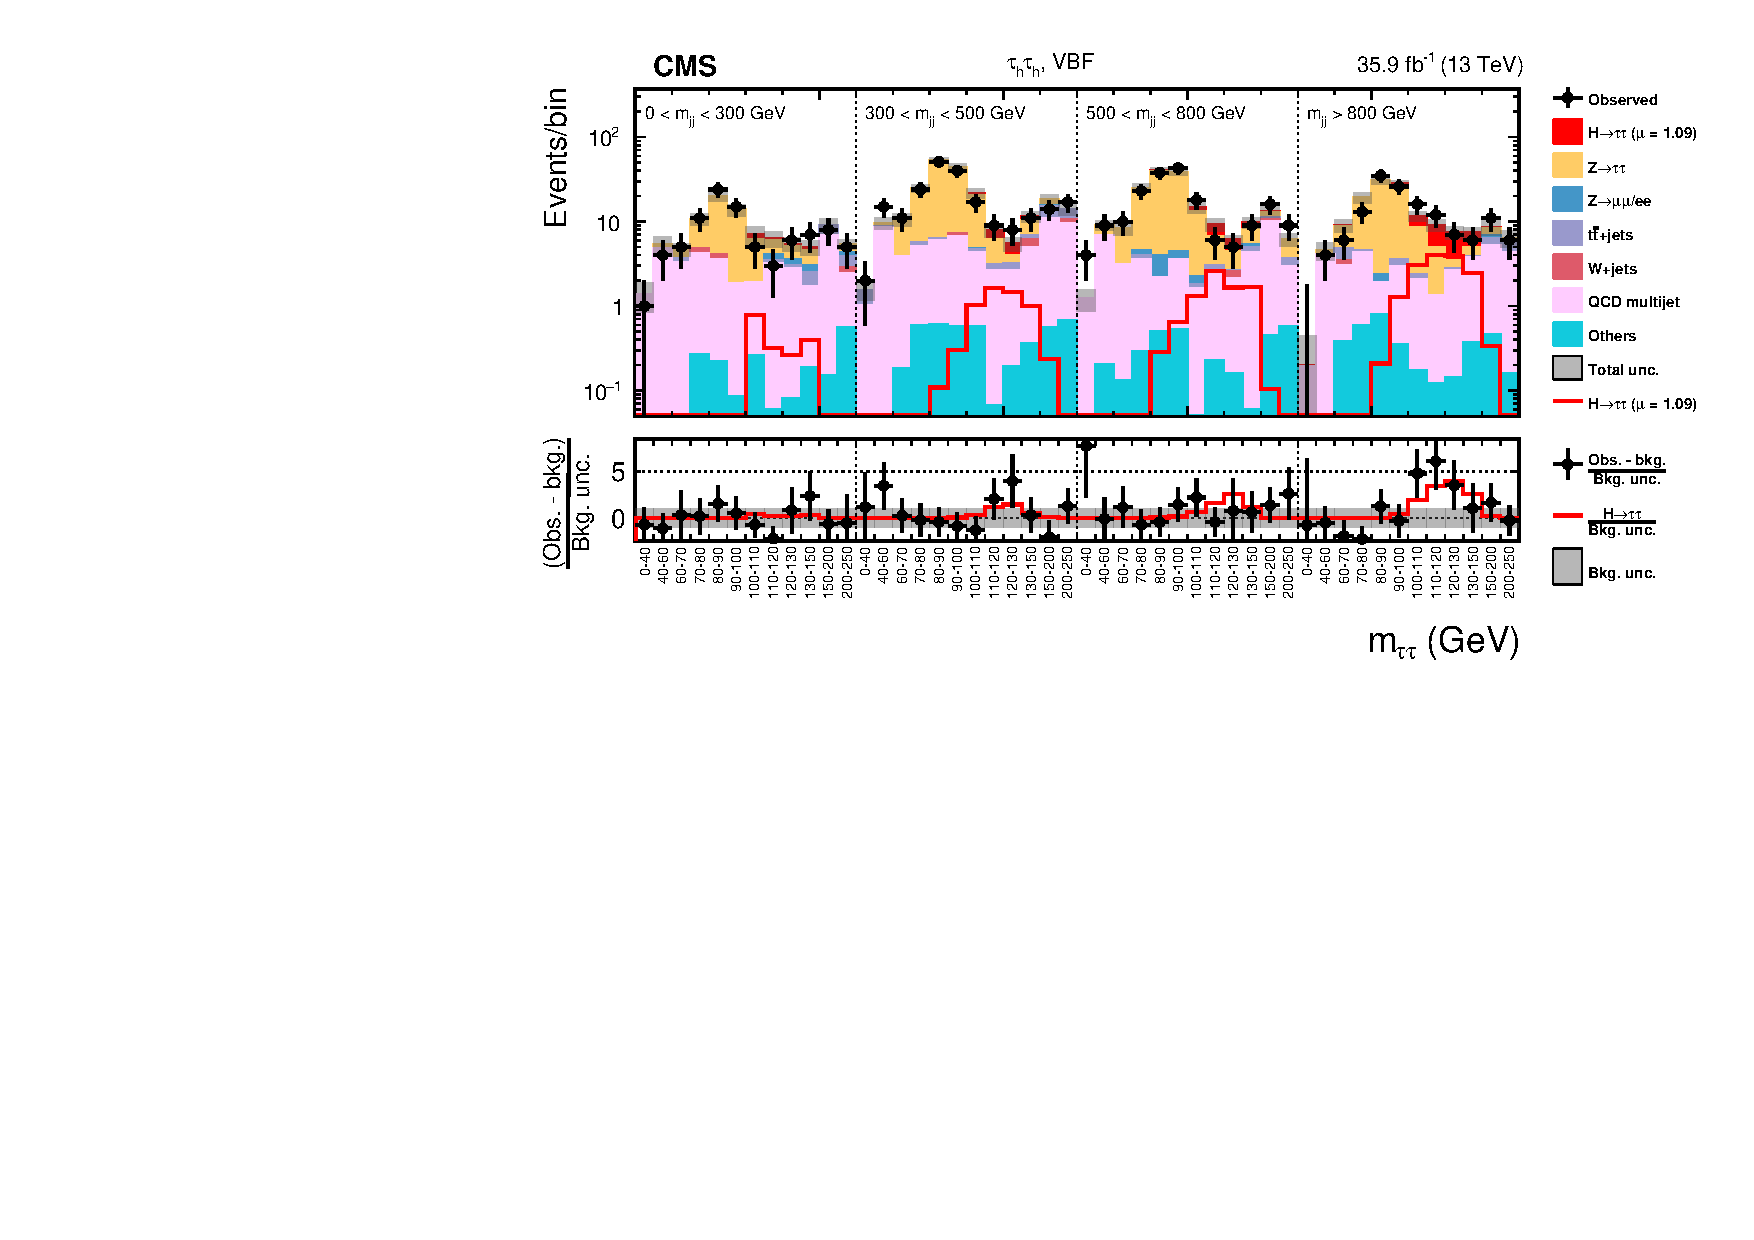
\includegraphics[width=1.0\textwidth]{figures/Figure_006.pdf}
     \caption{Observed and predicted 2D distributions in the VBF category of the $\tauh\tauh$ decay channel.
The normalization of the predicted background distributions corresponds to the result of the global fit.
The signal distribution is normalized to its best fit signal strength. The background histograms are stacked. The ``Others" background contribution includes events from diboson and single top quark production, as well as Higgs boson decays to a pair of $\PW$ bosons. The background uncertainty band accounts for all sources of background uncertainty, systematic as well as statistical, after the global fit. The signal is shown both as a stacked filled histogram and an open overlaid histogram.}
     \label{fig:mass_tt_0jet}
\end{figure*}

\begin{figure*}[htbp]
\centering
     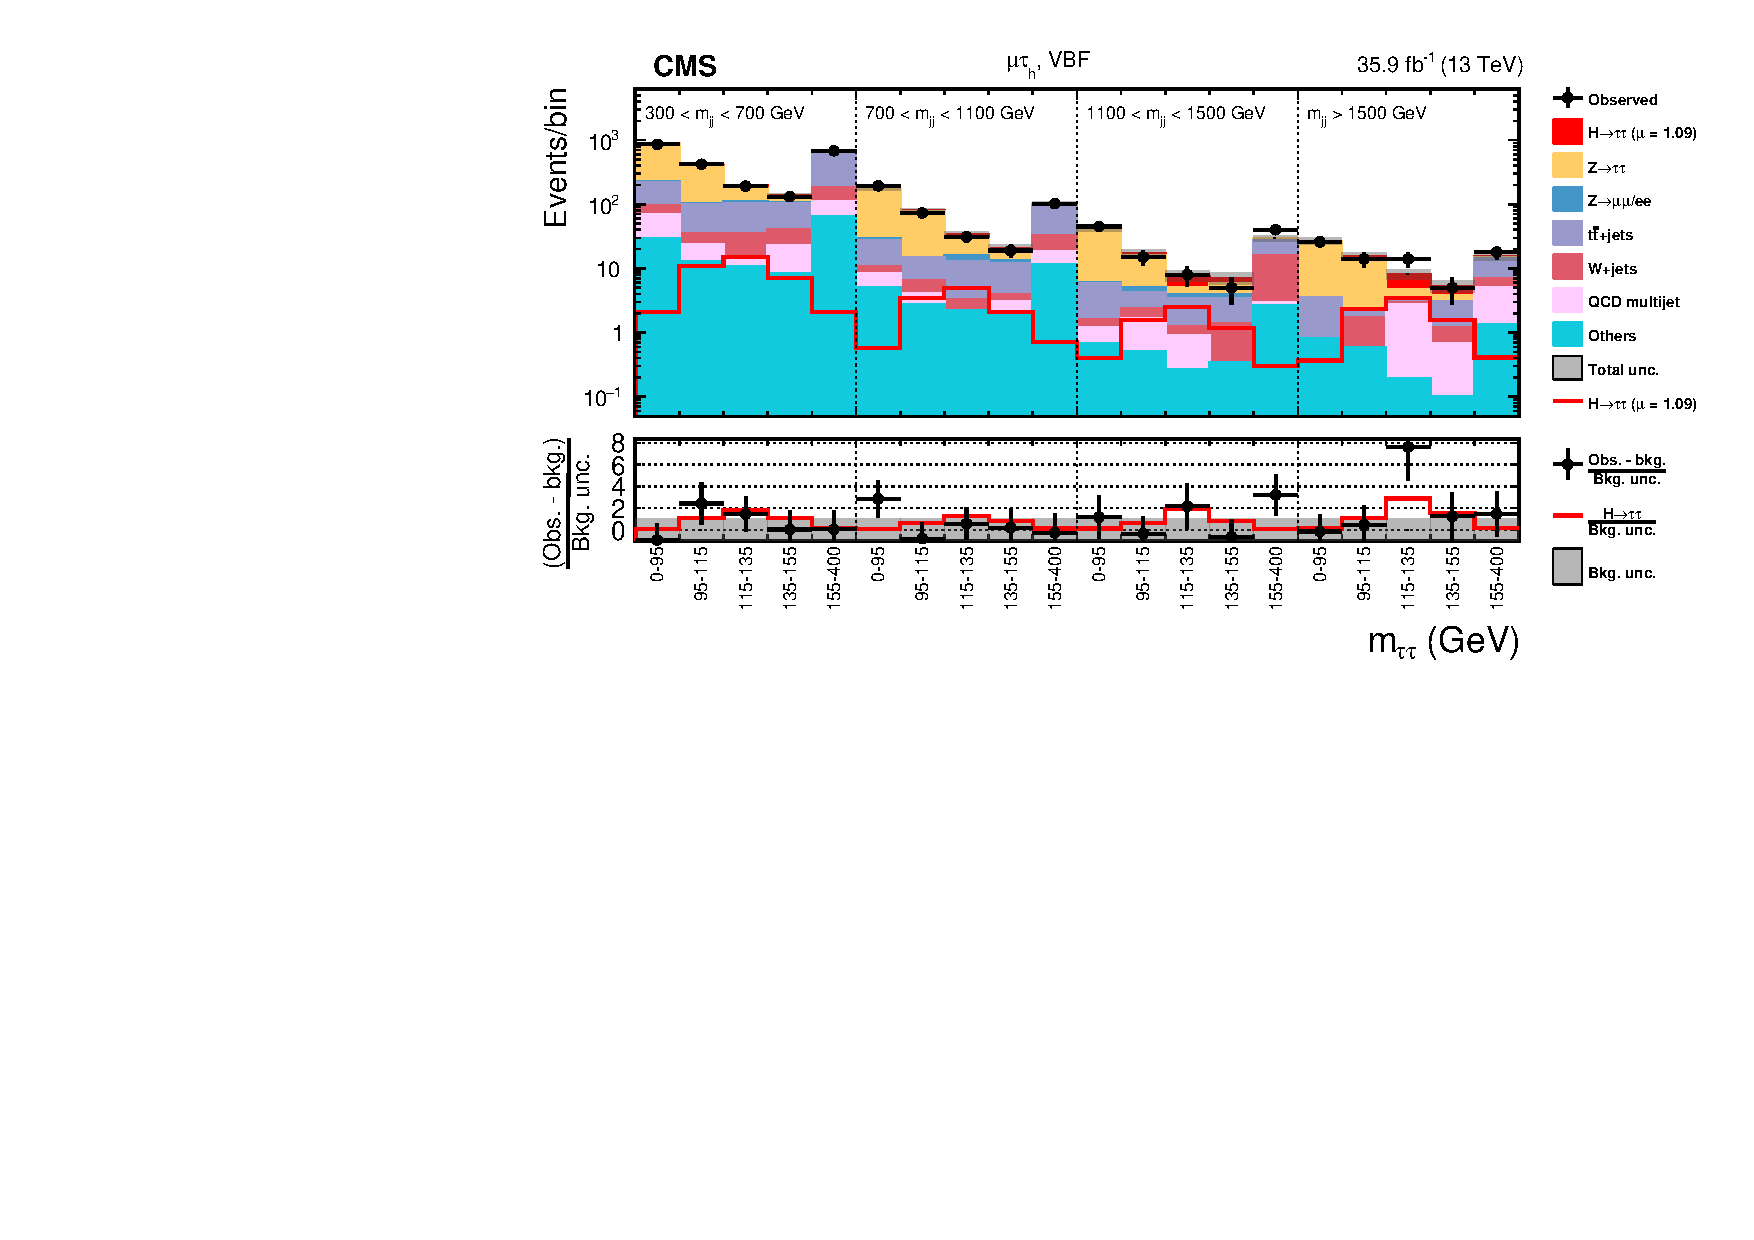
\includegraphics[width=1.0\textwidth]{figures/Figure_007.pdf}
     \caption{Observed and predicted 2D distributions in the VBF category of the $\Pgm\tauh$ decay channel. The description of the histograms is the same as in Fig.~\ref{fig:mass_tt_0jet}.}
     \label{fig:mass_tt_vbf}
\end{figure*}

\begin{figure*}[htbp]
\centering
     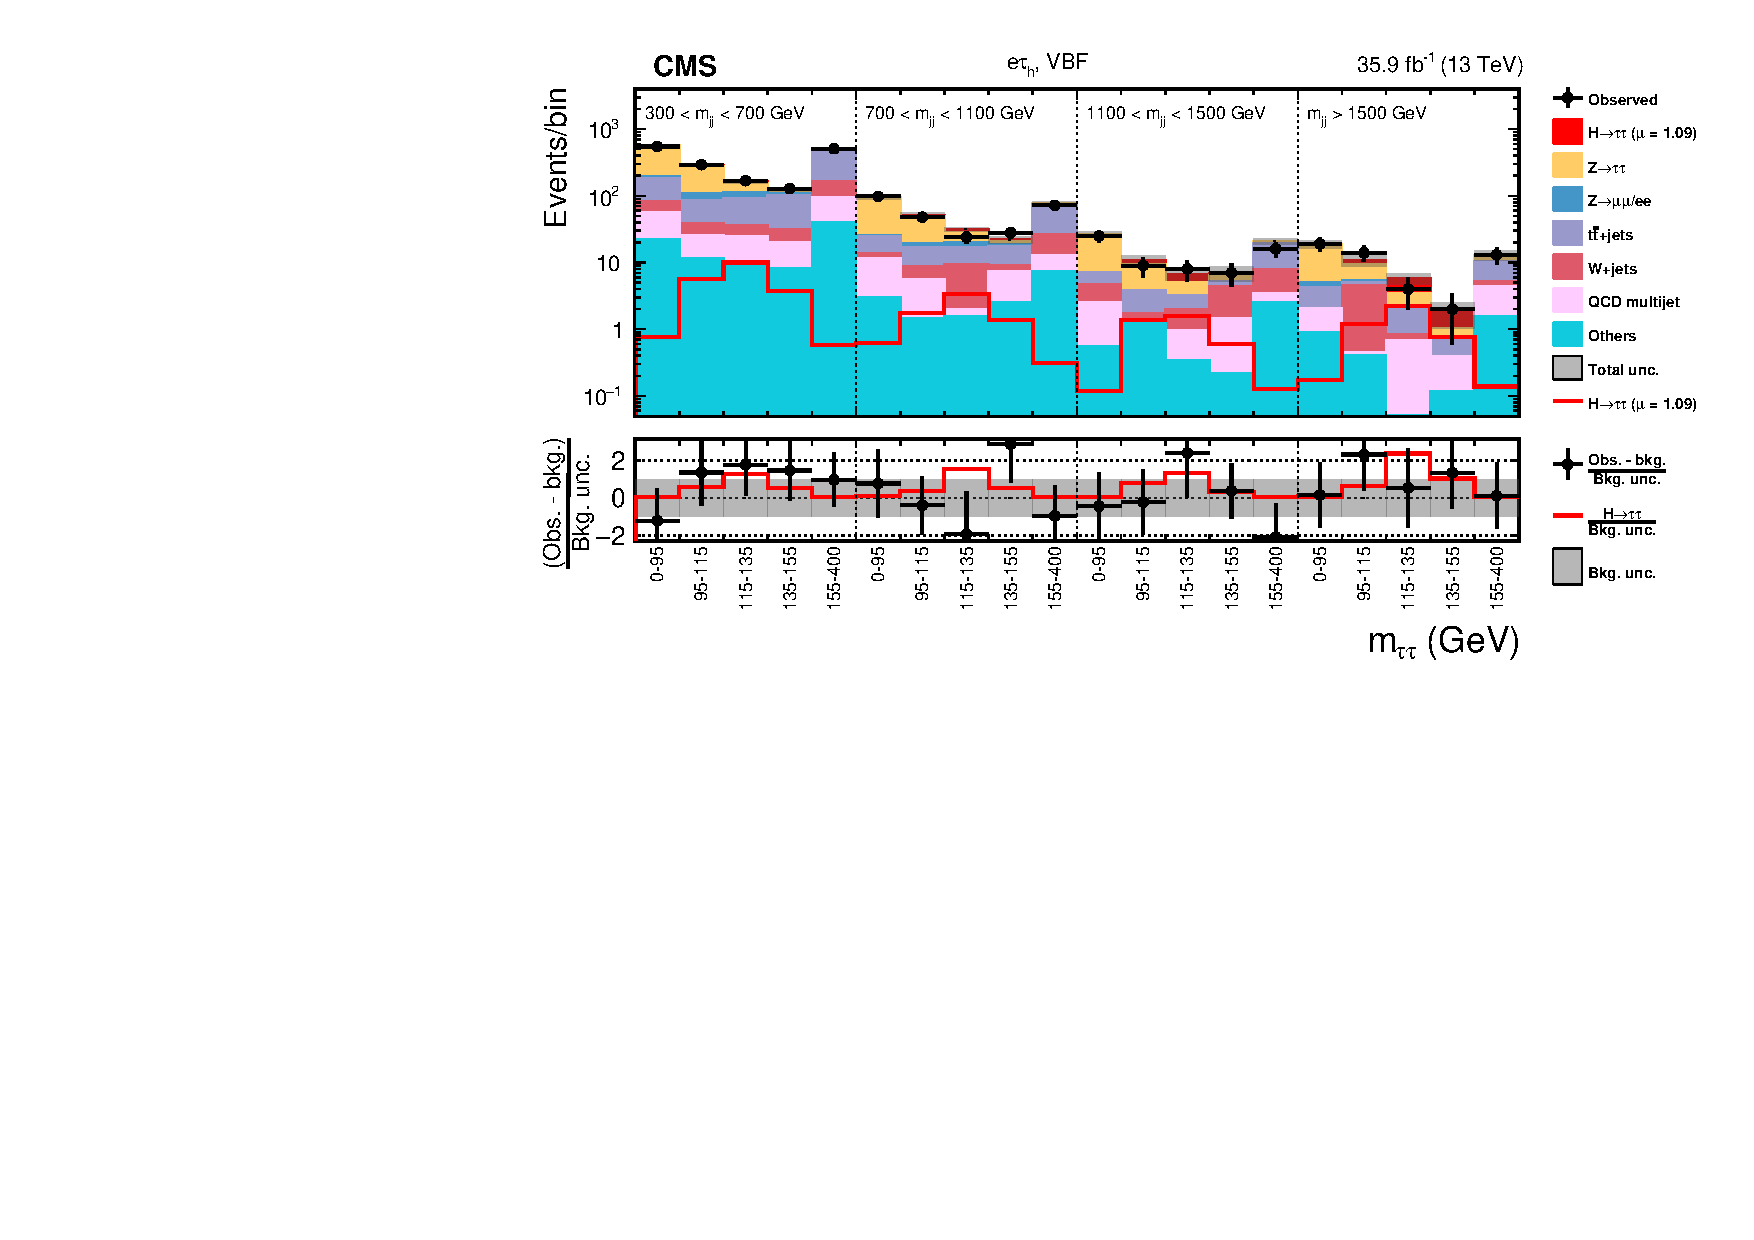
\includegraphics[width=1.0\textwidth]{figures/Figure_008.pdf}
     \caption{Observed and predicted 2D distributions in the VBF category of the $\Pe\tauh$ decay channel. The description of the histograms is the same as in Fig.~\ref{fig:mass_tt_0jet}.}
     \label{fig:mass_tt_boosted}
\end{figure*}


\begin{figure*}[htbp]
\centering
     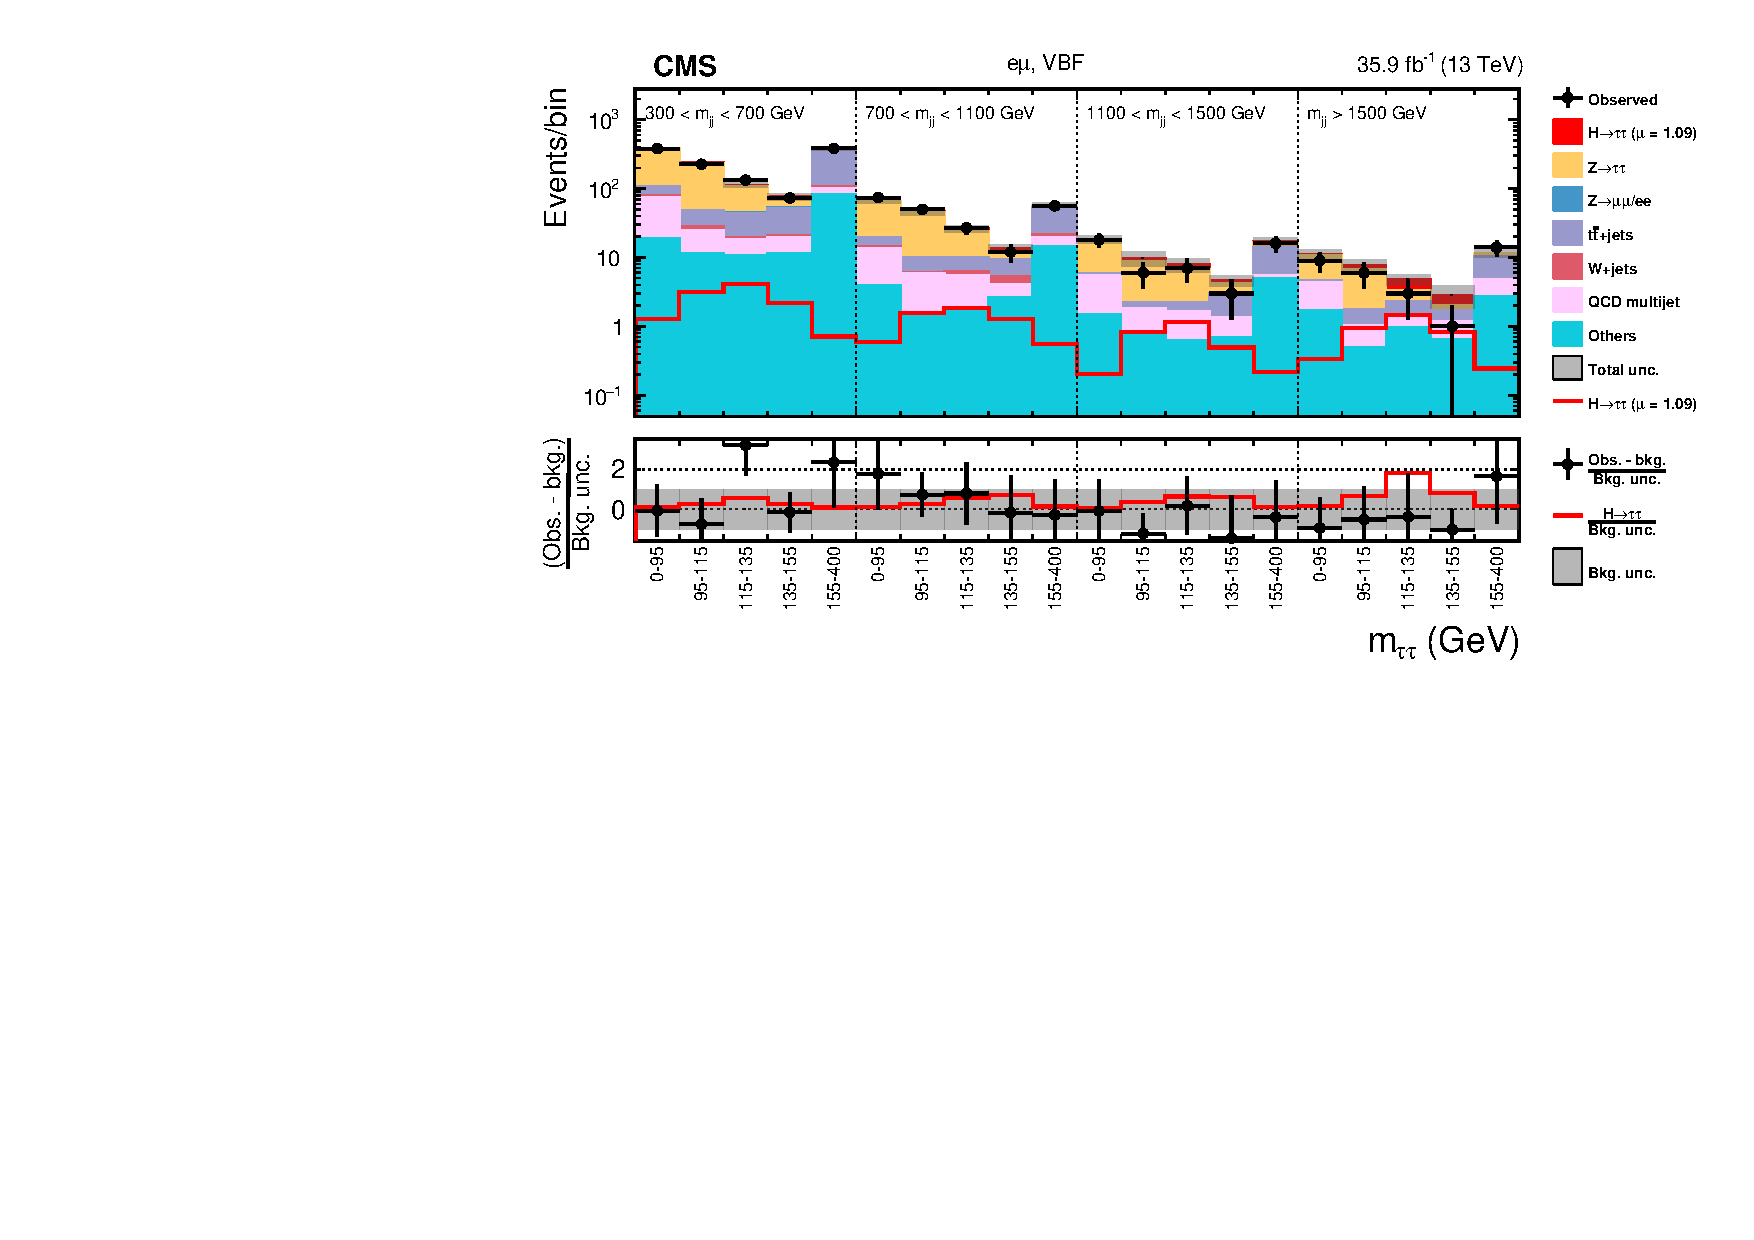
\includegraphics[width=1.0\textwidth]{figures/Figure_009.pdf}
     \caption{Observed and predicted 2D distributions in the VBF category of the $\Pe\Pgm$ decay channel. The description of the histograms is the same as in Fig.~\ref{fig:mass_tt_0jet}.}
     \label{fig:mass_mt_0jet}
\end{figure*}

\begin{figure*}[htbp]
\centering
     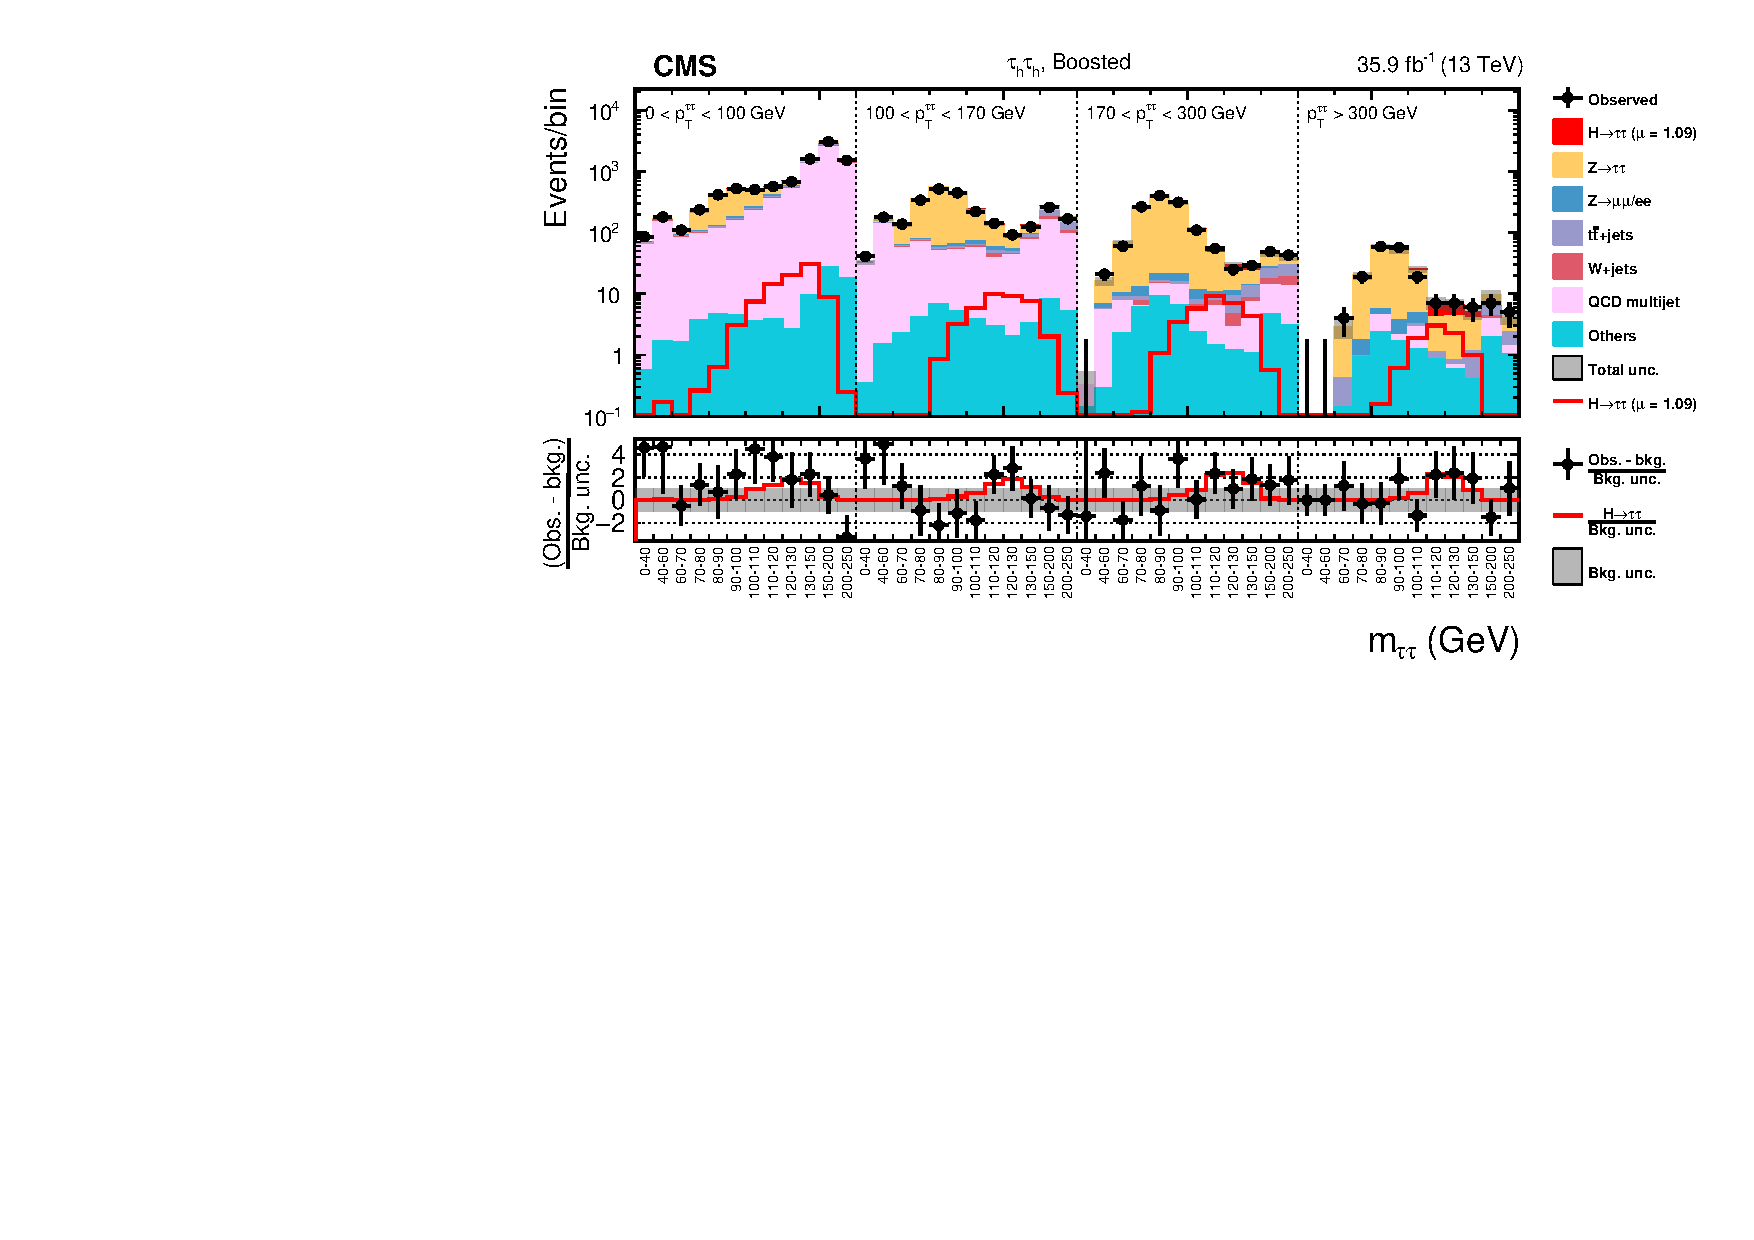
\includegraphics[width=1.0\textwidth]{figures/Figure_010.pdf}
     \caption{Observed and predicted 2D distributions in the boosted category of the $\tauh\tauh$ decay channel. The description of the histograms is the same as in Fig.~\ref{fig:mass_tt_0jet}.}
     \label{fig:mass_mt_vbf}
\end{figure*}

\begin{figure*}[htbp]
\centering
     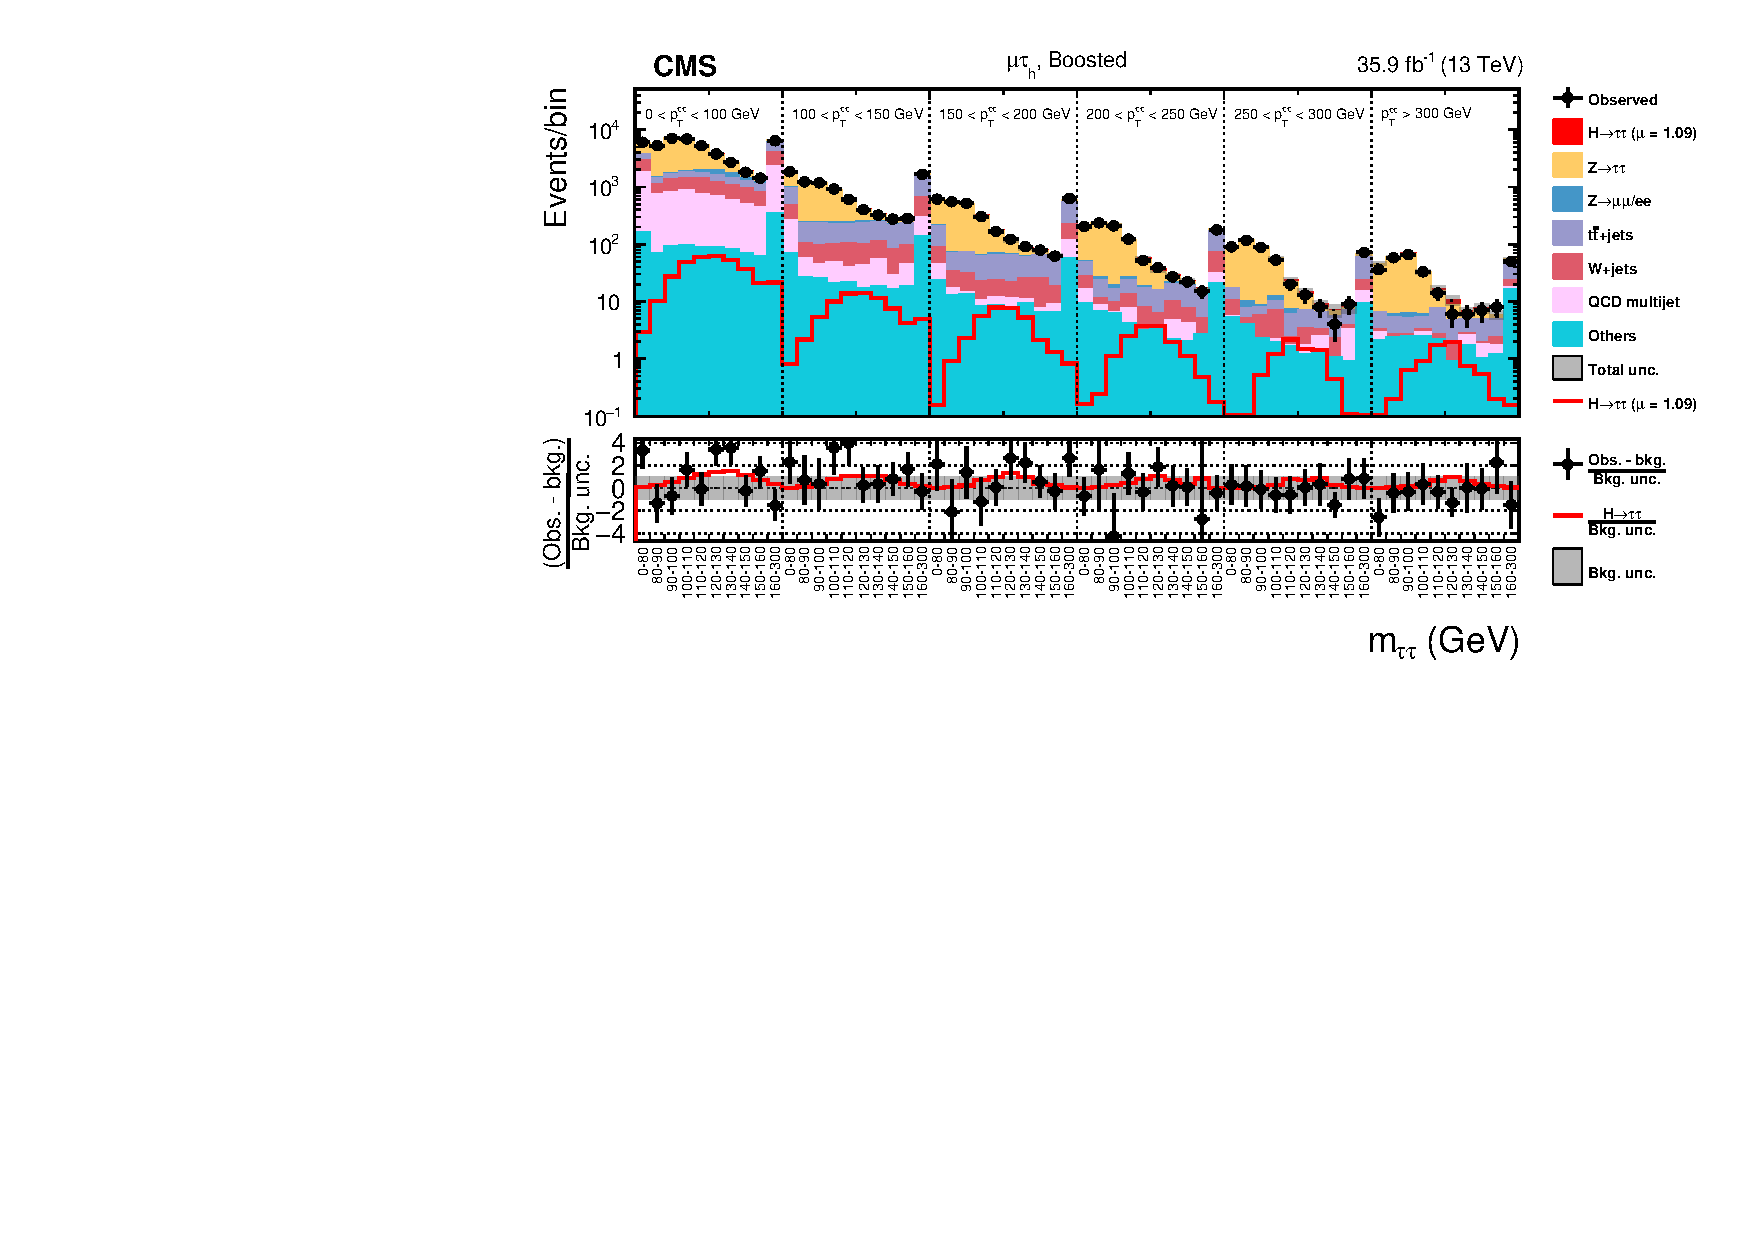
\includegraphics[width=1.0\textwidth]{figures/Figure_011.pdf}
     \caption{Observed and predicted 2D distributions in the boosted category of the $\Pgm\tauh$ decay channel. The description of the histograms is the same as in Fig.~\ref{fig:mass_tt_0jet}.}
     \label{fig:mass_mt_boosted}
\end{figure*}

\begin{figure*}[htbp]
\centering
     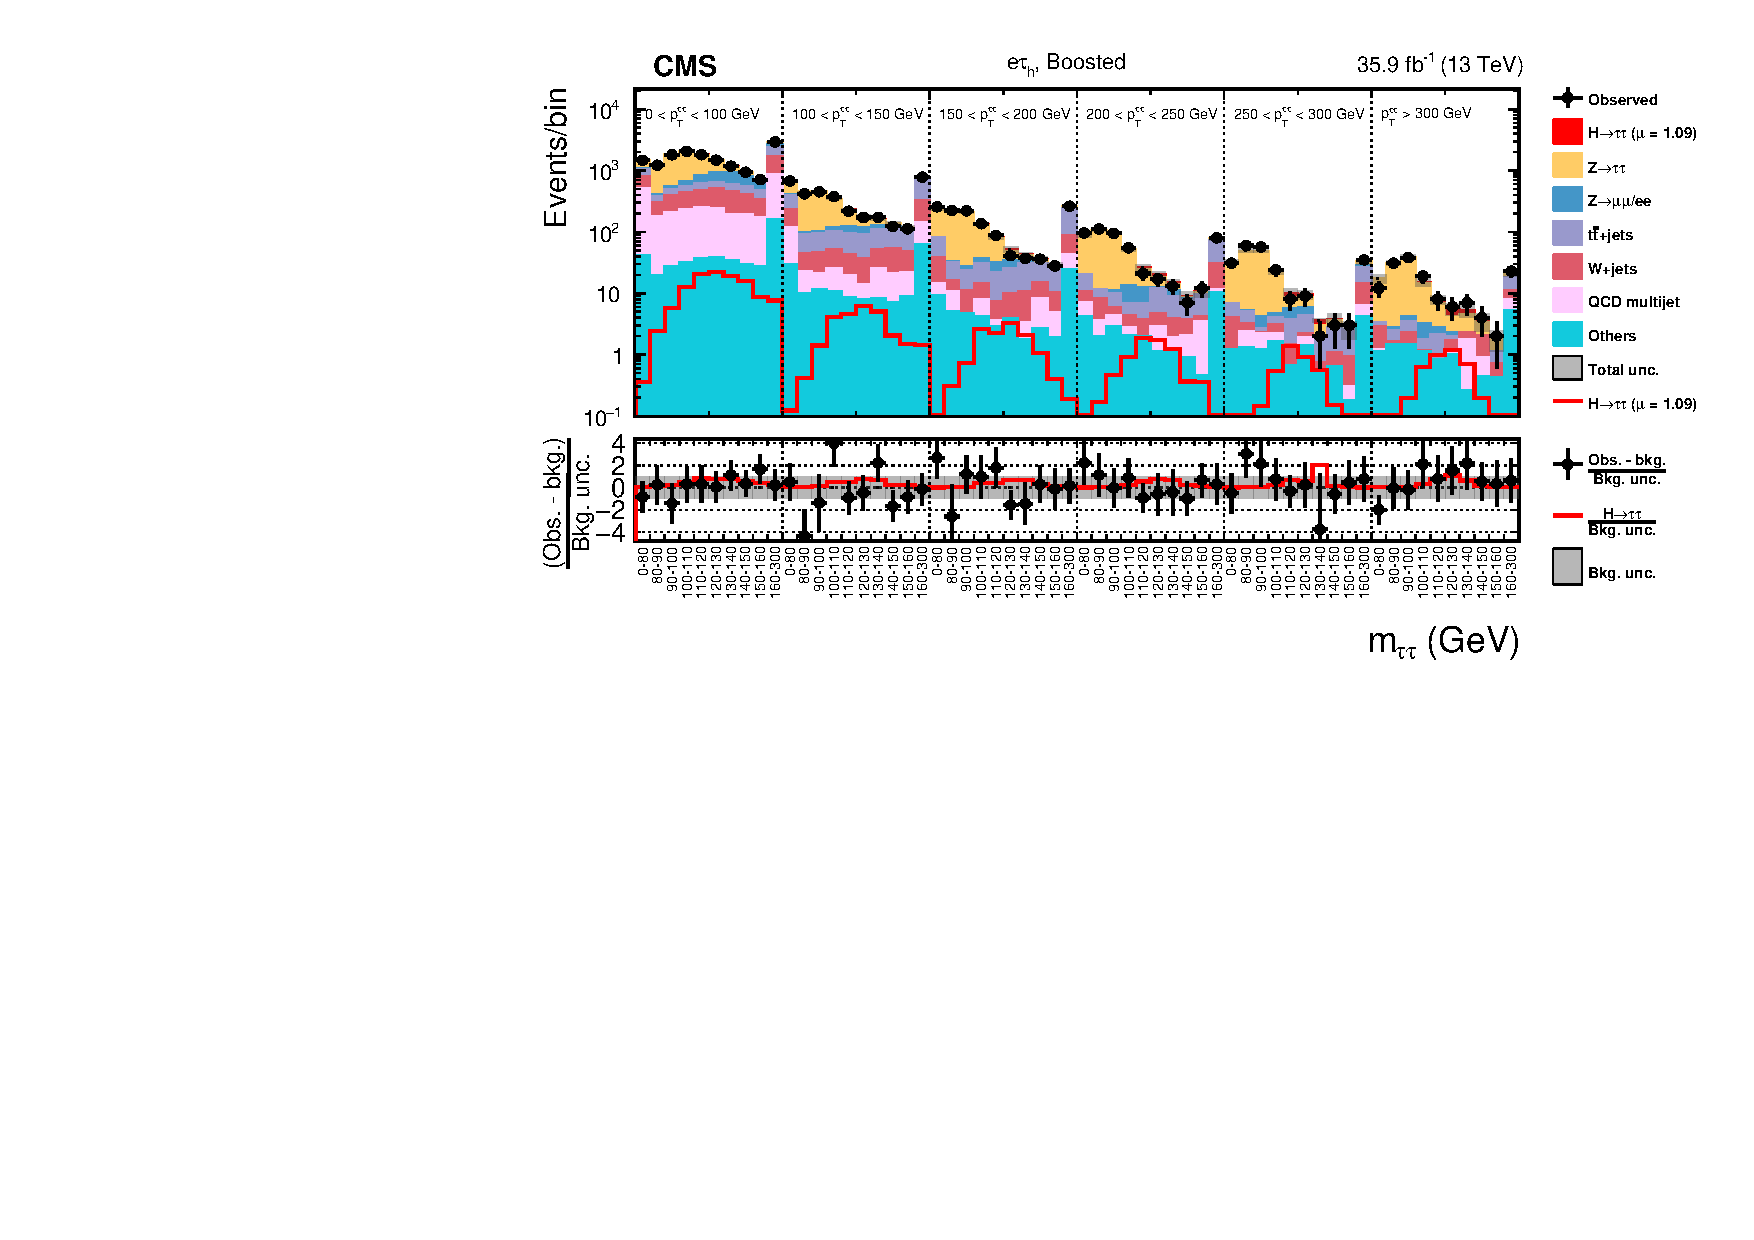
\includegraphics[width=1.0\textwidth]{figures/Figure_012.pdf}
     \caption{Observed and predicted 2D distributions in the boosted category of the $\Pe\tauh$ decay channel. The description of the histograms is the same as in Fig.~\ref{fig:mass_tt_0jet}.}
     \label{fig:mass_et_0jet}
\end{figure*}

\begin{figure*}[htbp]
\centering
     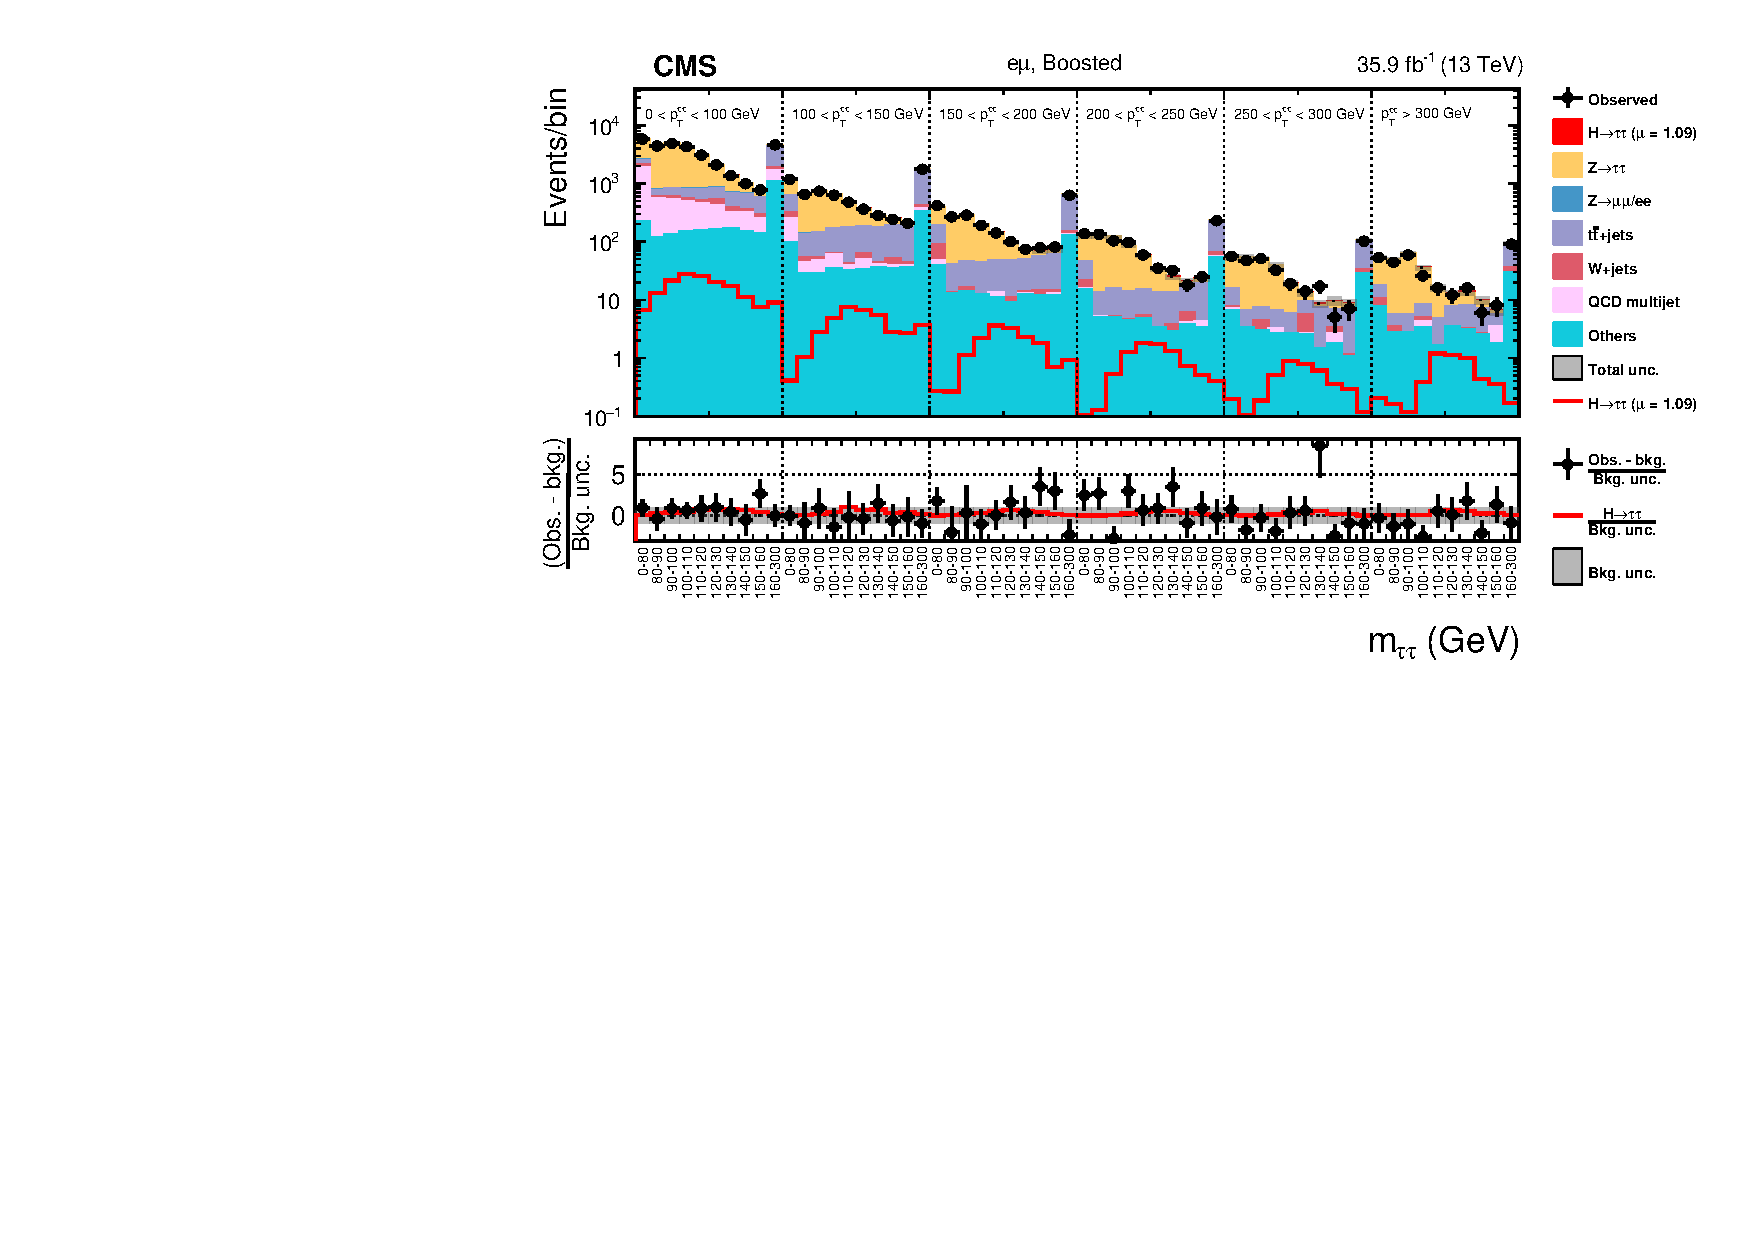
\includegraphics[width=1.0\textwidth]{figures/Figure_013.pdf}
     \caption{Observed and predicted 2D distributions in the boosted category of the $\Pe\Pgm$ decay channel. The description of the histograms is the same as in Fig.~\ref{fig:mass_tt_0jet}.}
     \label{fig:mass_et_vbf}
\end{figure*}

\begin{figure*}[htbp]
\centering
     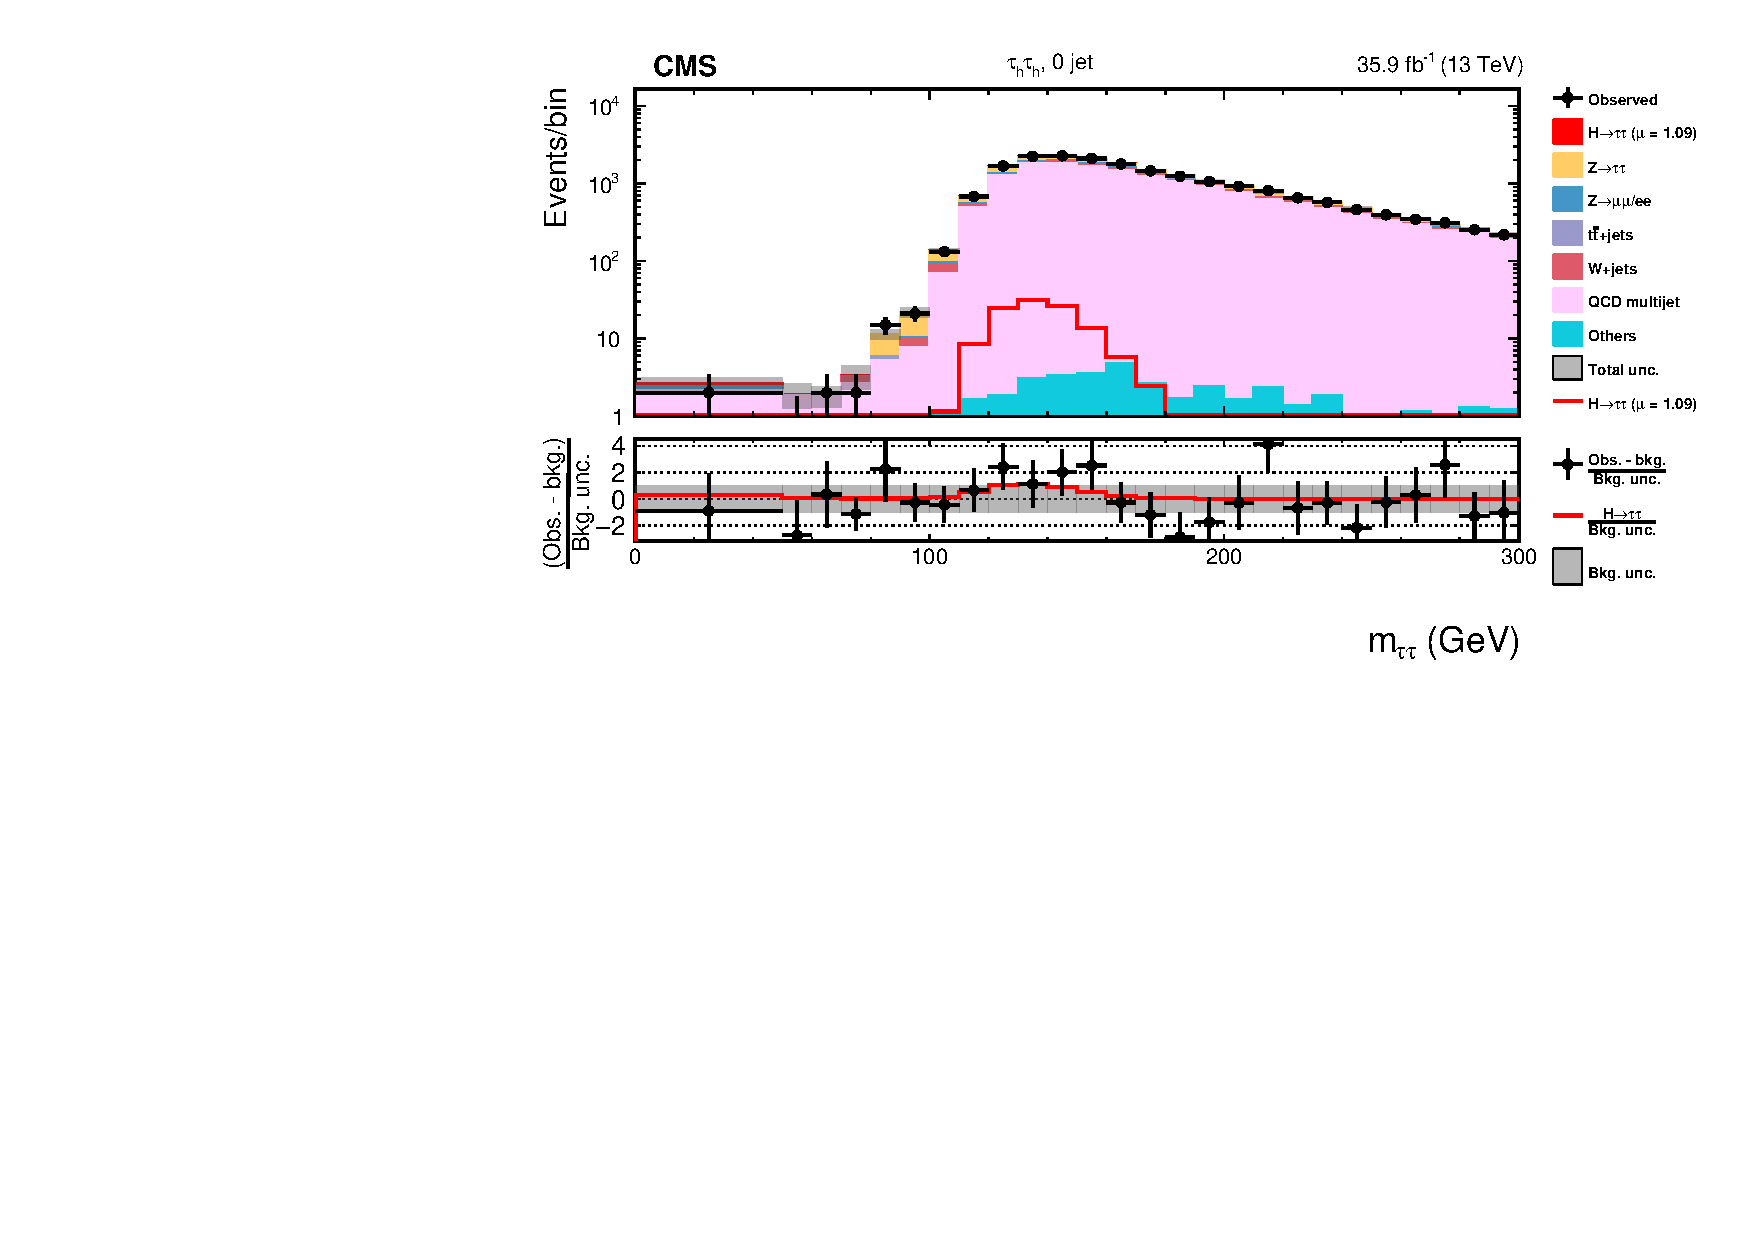
\includegraphics[width=1.0\textwidth]{figures/Figure_014.pdf}
     \caption{Observed and predicted distributions in the 0-jet category of the $\tauh\tauh$ decay channel. The description of the histograms is the same as in Fig.~\ref{fig:mass_tt_0jet}.}
     \label{fig:mass_et_boosted}
\end{figure*}



\begin{figure*}[htbp]
\centering
     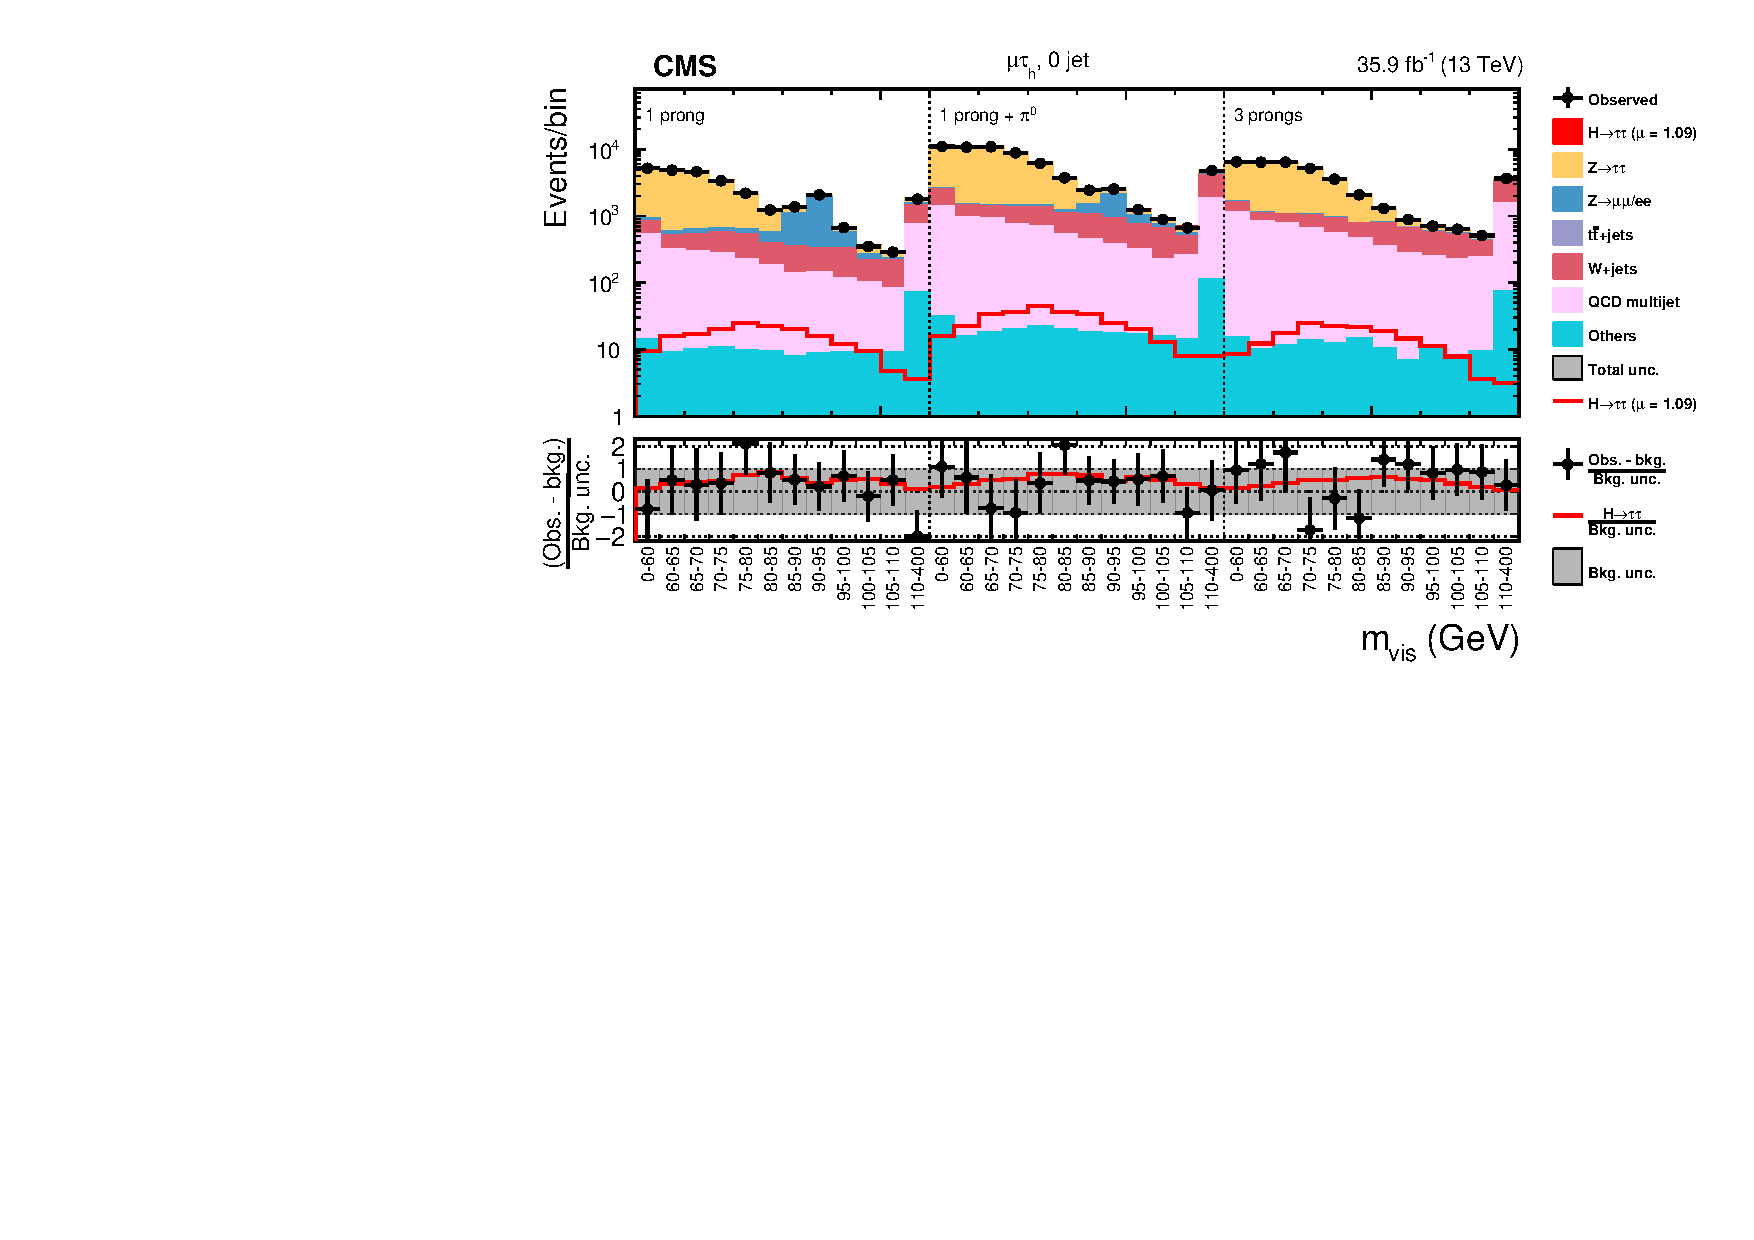
\includegraphics[width=1.0\textwidth]{figures/Figure_015.pdf}
     \caption{Observed and predicted 2D distributions in the 0-jet category of the $\Pgm\tauh$ decay channel. The description of the histograms is the same as in Fig.~\ref{fig:mass_tt_0jet}.}
     \label{fig:mass_em_0jet}
\end{figure*}

\begin{figure*}[htbp]
\centering
     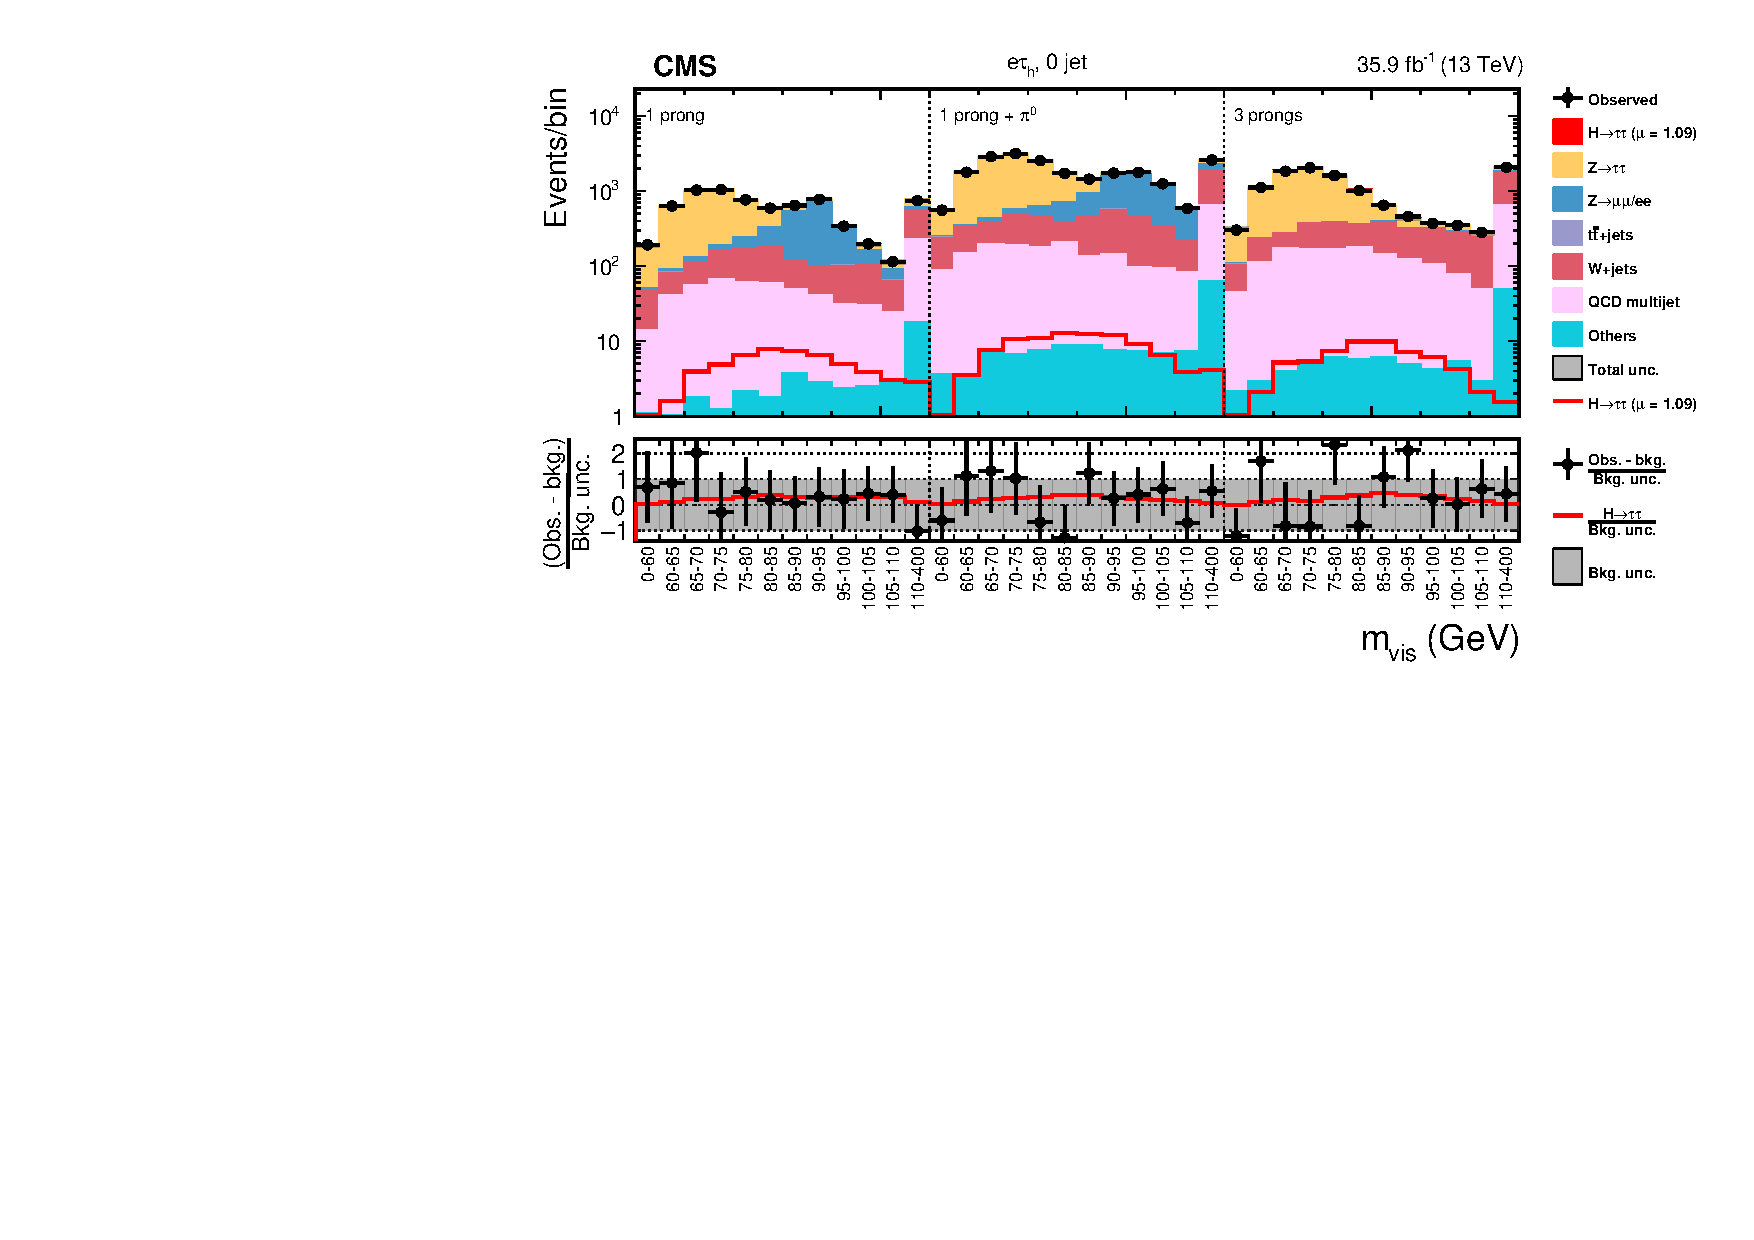
\includegraphics[width=1.0\textwidth]{figures/Figure_016.pdf}
     \caption{Observed and predicted 2D distributions in the 0-jet category of the $\Pe\tauh$ decay channel. The description of the histograms is the same as in Fig.~\ref{fig:mass_tt_0jet}.}
     \label{fig:mass_em_vbf}
\end{figure*}

\begin{figure*}[htbp]
\centering
     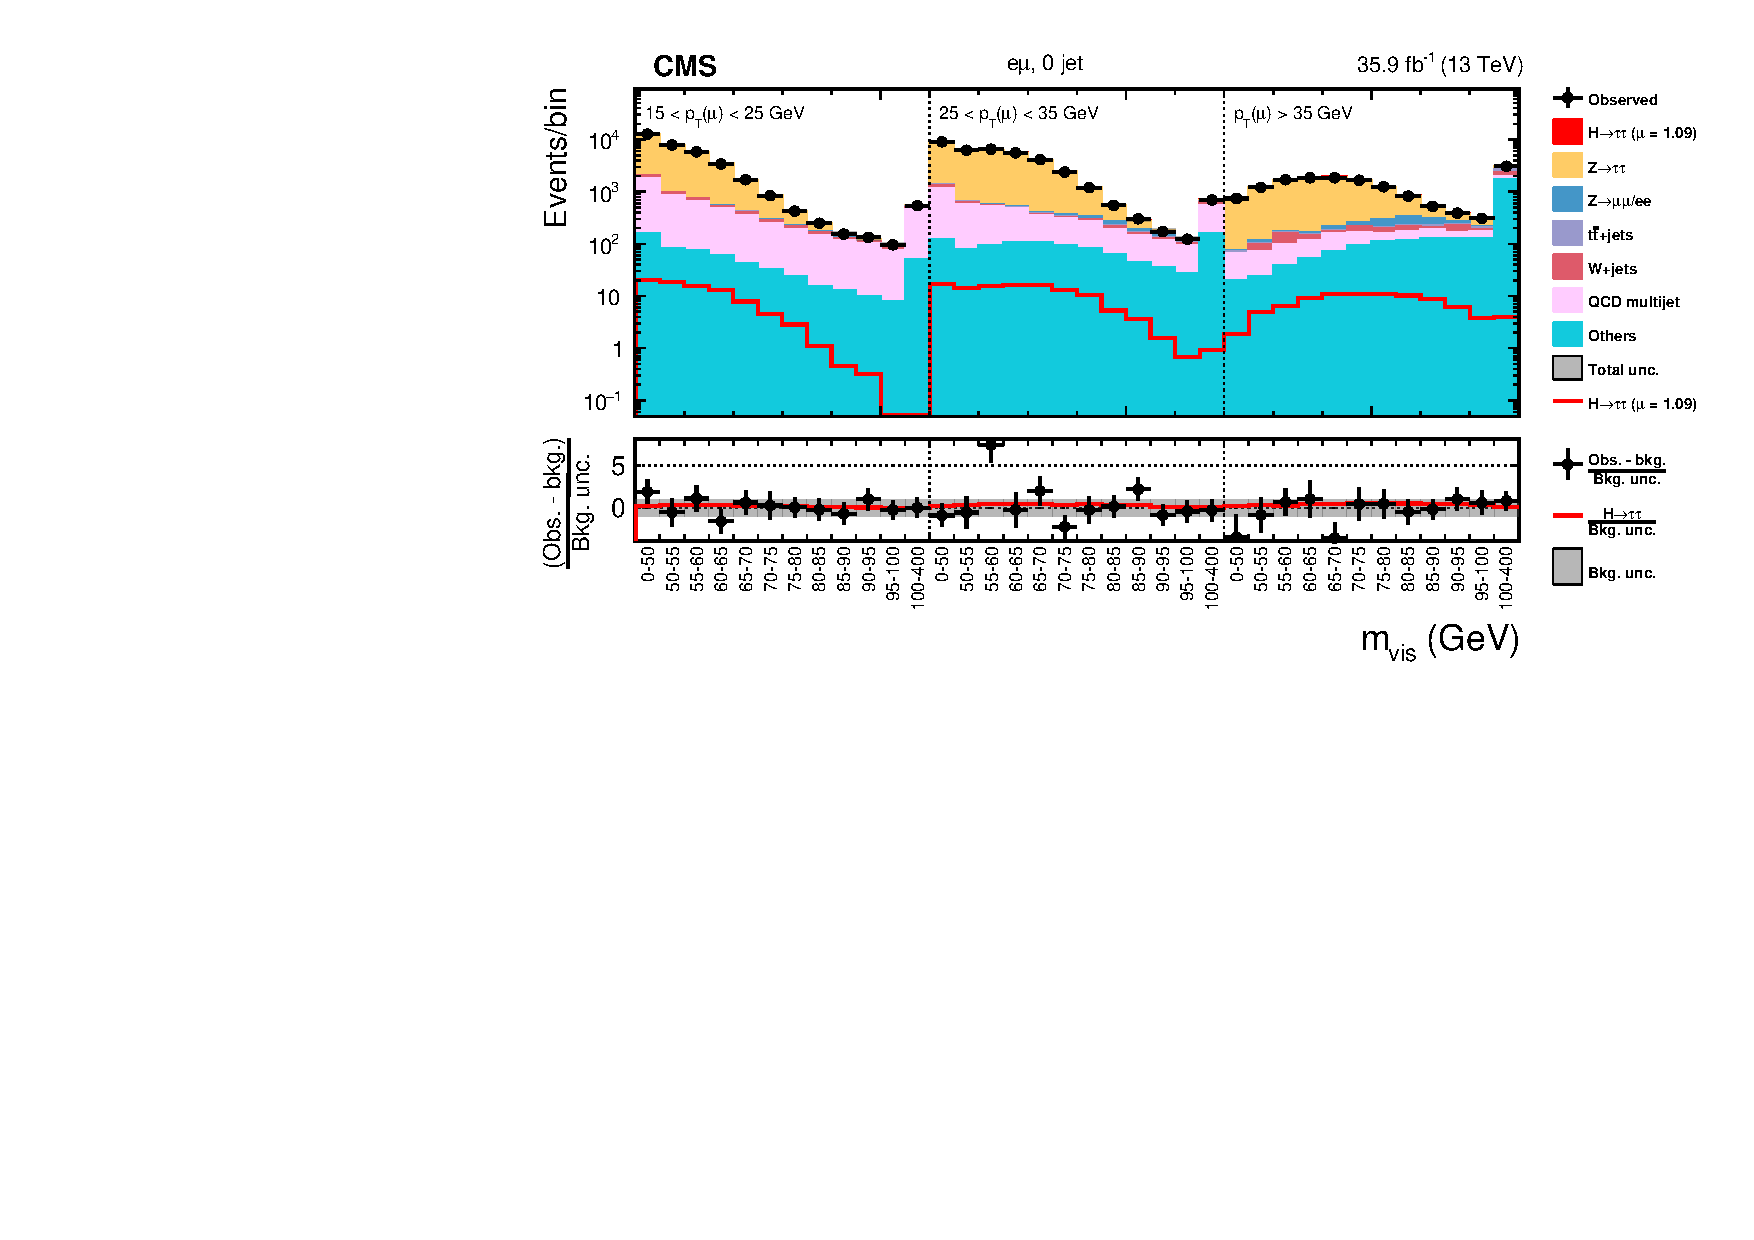
\includegraphics[width=1.0\textwidth]{figures/Figure_017.pdf}
     \caption{Observed and predicted 2D distributions in the 0-jet category of the $\Pe\Pgm$ decay channel. The description of the histograms is the same as in Fig.~\ref{fig:mass_tt_0jet}.}
     \label{fig:mass_em_boosted}
\end{figure*}


The 2D distributions of the final discriminating variables obtained for each category and each channel in the signal regions, along with the control regions, are combined in a binned likelihood involving the expected and observed numbers of events in each bin.
The expected number of signal events is the one predicted for the production of
a SM Higgs boson of mass $\mH=125.09\GeV$ decaying into a pair of $\Pgt$ leptons,
multiplied by a signal strength modifier $\mu$ treated as a free parameter in the fit.

The systematic uncertainties are represented by nuisance parameters that are varied in the fit according to their probability density functions.
A log-normal probability density function is assumed for the nuisance parameters affecting the event yields of the various background contributions, whereas systematic uncertainties that affect the shape of the distributions are represented by nuisance parameters whose variation results in a continuous perturbation of the spectrum~\cite{Conway-PhyStat} and which are assumed to have a Gaussian probability density function.
Overall, the statistical uncertainty in the observed event yields is the dominant source of uncertainty for all combined results.

Grouping events
in the signal region by their decimal logarithm of the ratio of the signal ($S$) to signal-plus-background ($S+B$) in each bin (Fig.~\ref{fig:sb}), an excess of observed events with respect to the SM background expectation is clearly visible in the most sensitive bins of the analysis. The expected background and signal contributions, as well as the observed number of events, are indicated per process and category in Table~\ref{tab:sb} for the bins with $\log_{10}(S/(S+B))>-0.9$. The channel that contributes the most to these bins is $\tauh\tauh$.

\begin{figure}[htb]
  \centering
    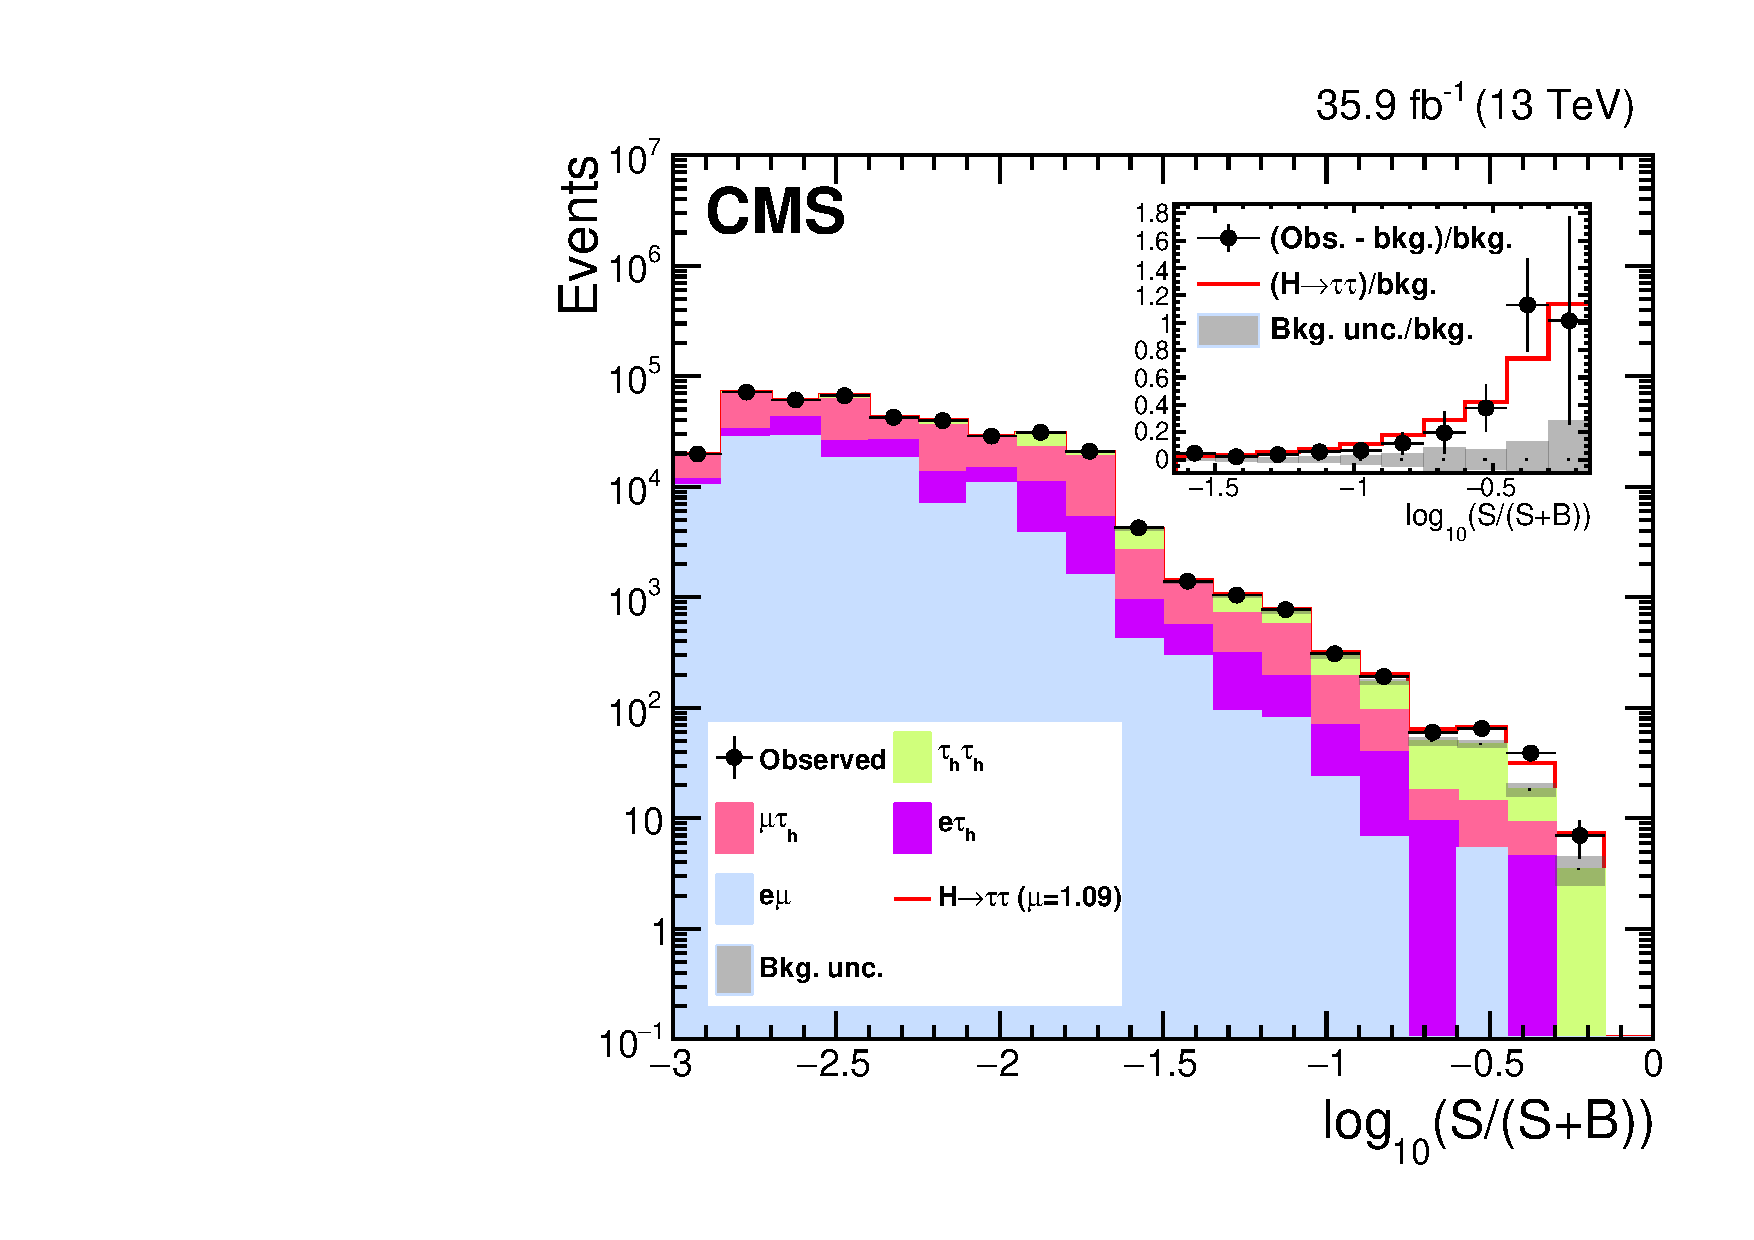
\includegraphics[width=0.65\textwidth]{figures/Figure_018.pdf}
   \caption{Distribution of the decimal logarithm of the ratio between the expected signal and the sum of expected signal and expected background in each bin of the mass distributions used to extract the results, in all signal regions. The background contributions are separated by decay channel. The inset shows the corresponding difference between the observed data and expected background distributions divided by the background expectation, as well as the signal expectation divided by the background expectation.
   }
    \label{fig:sb}

\end{figure}

\begin{table*}
\centering
\label{tab:sb}
\newcolumntype{x}{D{,}{\,\pm\,}{4.2}}
\begin{tabular}{lxxxx}
Process & \multicolumn{1}{c}{$\Pe\Pgm$} &  \multicolumn{1}{c}{$\Pe\tauh$} &  \multicolumn{1}{c}{$\Pgm\tauh$} &  \multicolumn{1}{c}{$\tauh\tauh$} \\
\hline
$\PZ \to\Pgt\Pgt$ & 5.8, 2.2 & 21.2, 3.3 &34.6, 4.9 & 89.1, 6.9 \\
$\PZ \to \Pe\Pe/\Pgm\Pgm$ & 0.0, 0.0 & 2.9, 0.2 &3.7, 0.2 & 5.0, 0.2 \\
$\ttbar$+jets & 1.9, 0.1 & 10.4, 0.3 &22.2, 1.8 & 13.9, 0.5 \\
$\PW+\text{jets}$ & 0.8, 0.02 & 4.0, 0.3 &6.6, 1.3 & 7.6, 0.8 \\
QCD multijet & 2.1, 0.3 & 3.3, 2.5 &5.0, 1.3 & 35.5, 2.1 \\
Other backgrounds & 1.4, 0.1 & 5.2, 0.2 &6.1, 0.2 & 7.3, 0.2 \\[\cmsTabSkip]
$\Pgg\Pgg\PH, \PH \to\Pgt\Pgt$ & 0.6, 0.1 & 5.0, 0.6 &6.0, 0.6 & 27.4, 2.1  \\
VBF $\PH \to\Pgt\Pgt$ & 2.8, 0.3 & 5.1, 0.5 &12.55, 1.0 & 17.5, 1.0 \\
V$\PH, \PH \to\Pgt\Pgt$ & 0.0, 0.0 & 0.3, 0.0 &0.2, 0.0 & 1.3, 0.1  \\[\cmsTabSkip]
Total backgrounds & 12.1, 2.2 & 46.5, 4.1 &77.7, 5.5 & 156.2, 7.3 \\
Total signal & 3.4, 0.4 & 10.9, 0.8 &19.2, 1.4 & 48.3, 2.6  \\
Observed &  \multicolumn{1}{c}{11} &  \multicolumn{1}{c}{54} &  \multicolumn{1}{c}{91} &  \multicolumn{1}{c}{207}  \\
\hline
\end{tabular}
\caption{Background and signal expectations, together with the number of observed events, for bins in the signal region for which $\log_{10}(S/(S+B))>-0.9$, where
$S$ and $B$ are, respectively, the number of expected signal events for a Higgs boson with a mass $\mH = 125.09$\GeV and of expected background events, in those bins. The background uncertainty accounts for all sources of background uncertainty, systematic as well as statistical, after the global fit. The contribution from ``other backgrounds" includes events from diboson and single top quark production. The contribution from Higgs boson decays to a pair of $\PW$ bosons is zero in these bins.}
\end{table*}

An excess of observed events relative to the background expectation is also visible in Fig.~\ref{fig:massweighted}, where every mass distribution for a constant range of the second dimension of the signal distributions has been summed with a weight of $S/(S+B)$  to increase the contribution of the most sensitive distributions. In this case, $S$ and $B$ are computed, respectively, as the signal or background contribution in the mass distribution excluding the first and last bins, in which the amount of signal is negligible. The signal regions that use $\mvis$ instead of $\mtt$, namely the 0-jet category of the $\Pgm\tauh$, $\Pe\tauh$ and $\Pe\Pgm$ channels, are not included. The two panes of Fig.~\ref{fig:massweighted} group the compatible bins of Figs.~\ref{fig:mass_tt_0jet}--\ref{fig:mass_em_boosted}.

\begin{figure}[htb]
  \centering
    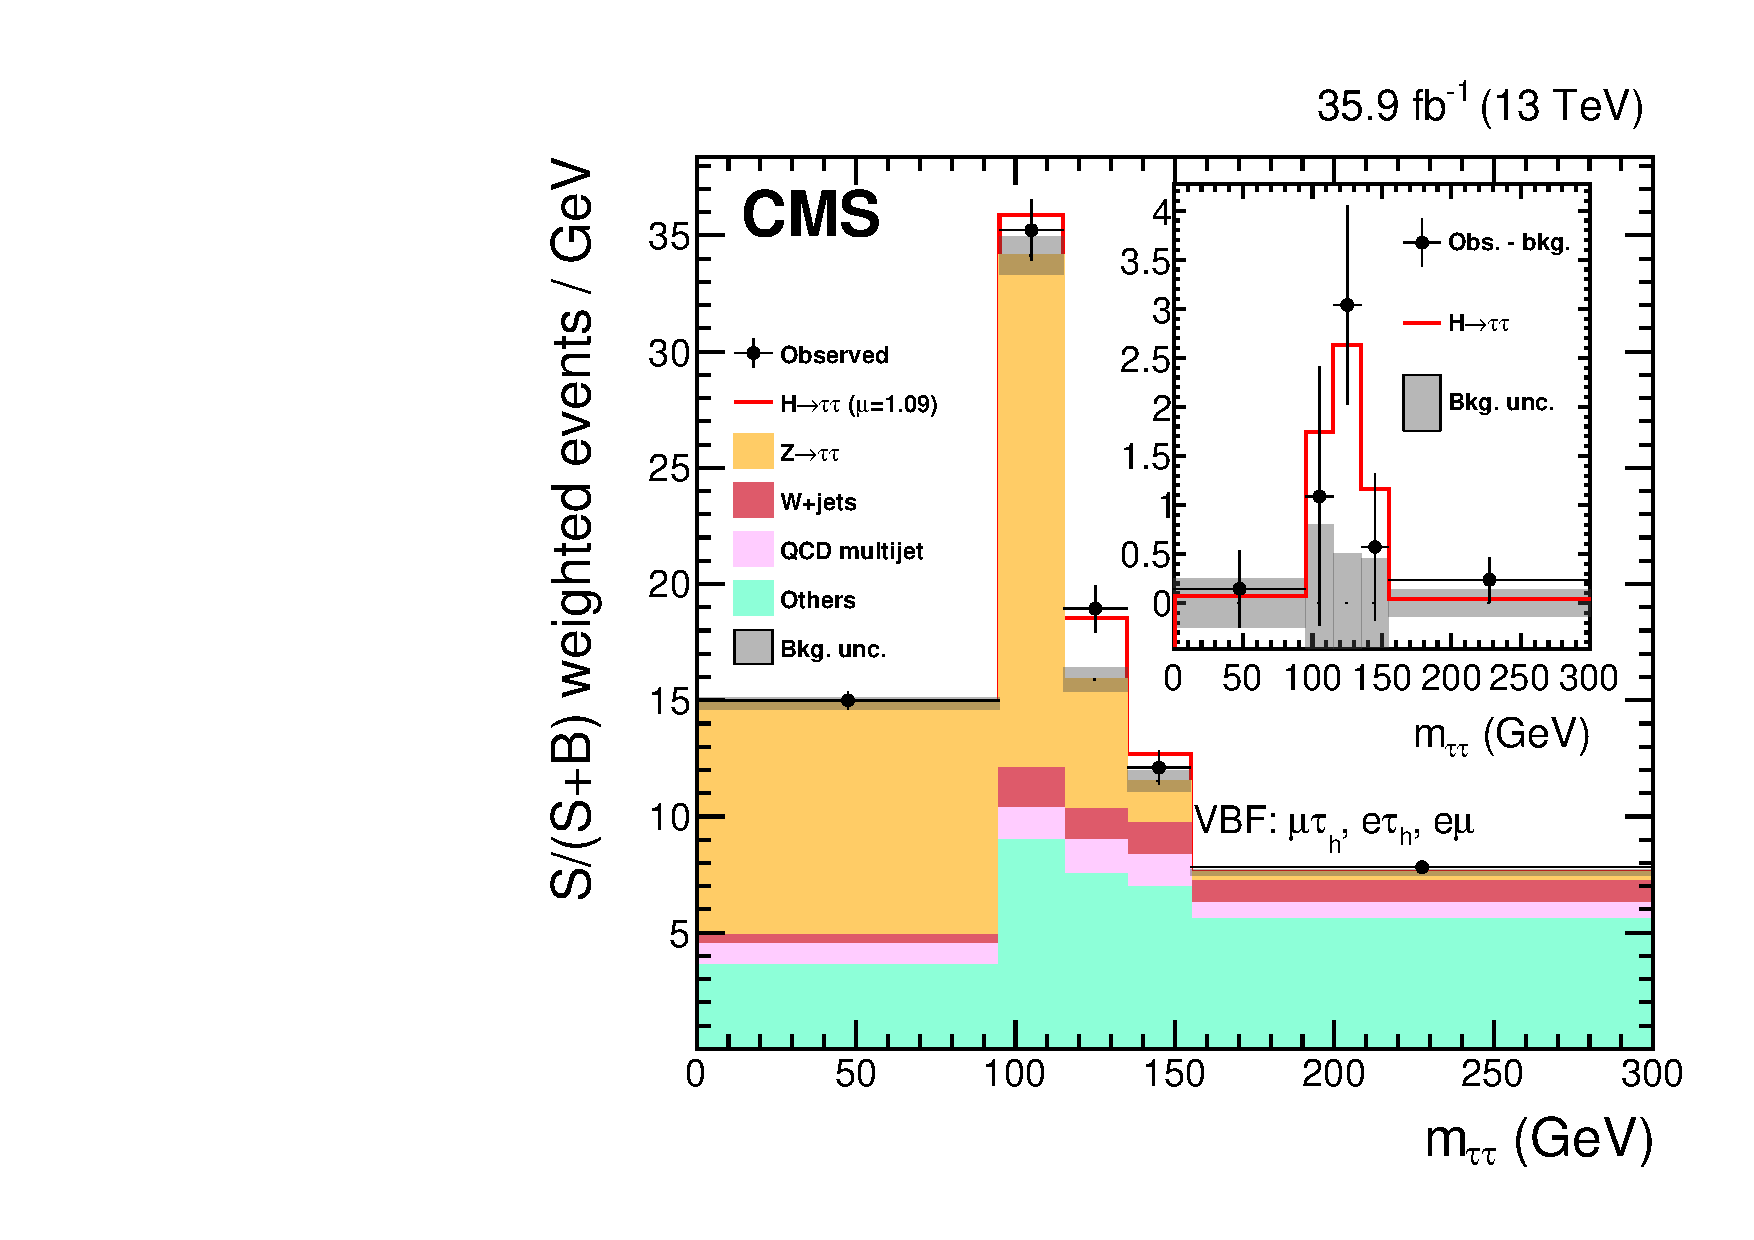
\includegraphics[width=0.48\textwidth]{figures/Figure_019-a.pdf}
    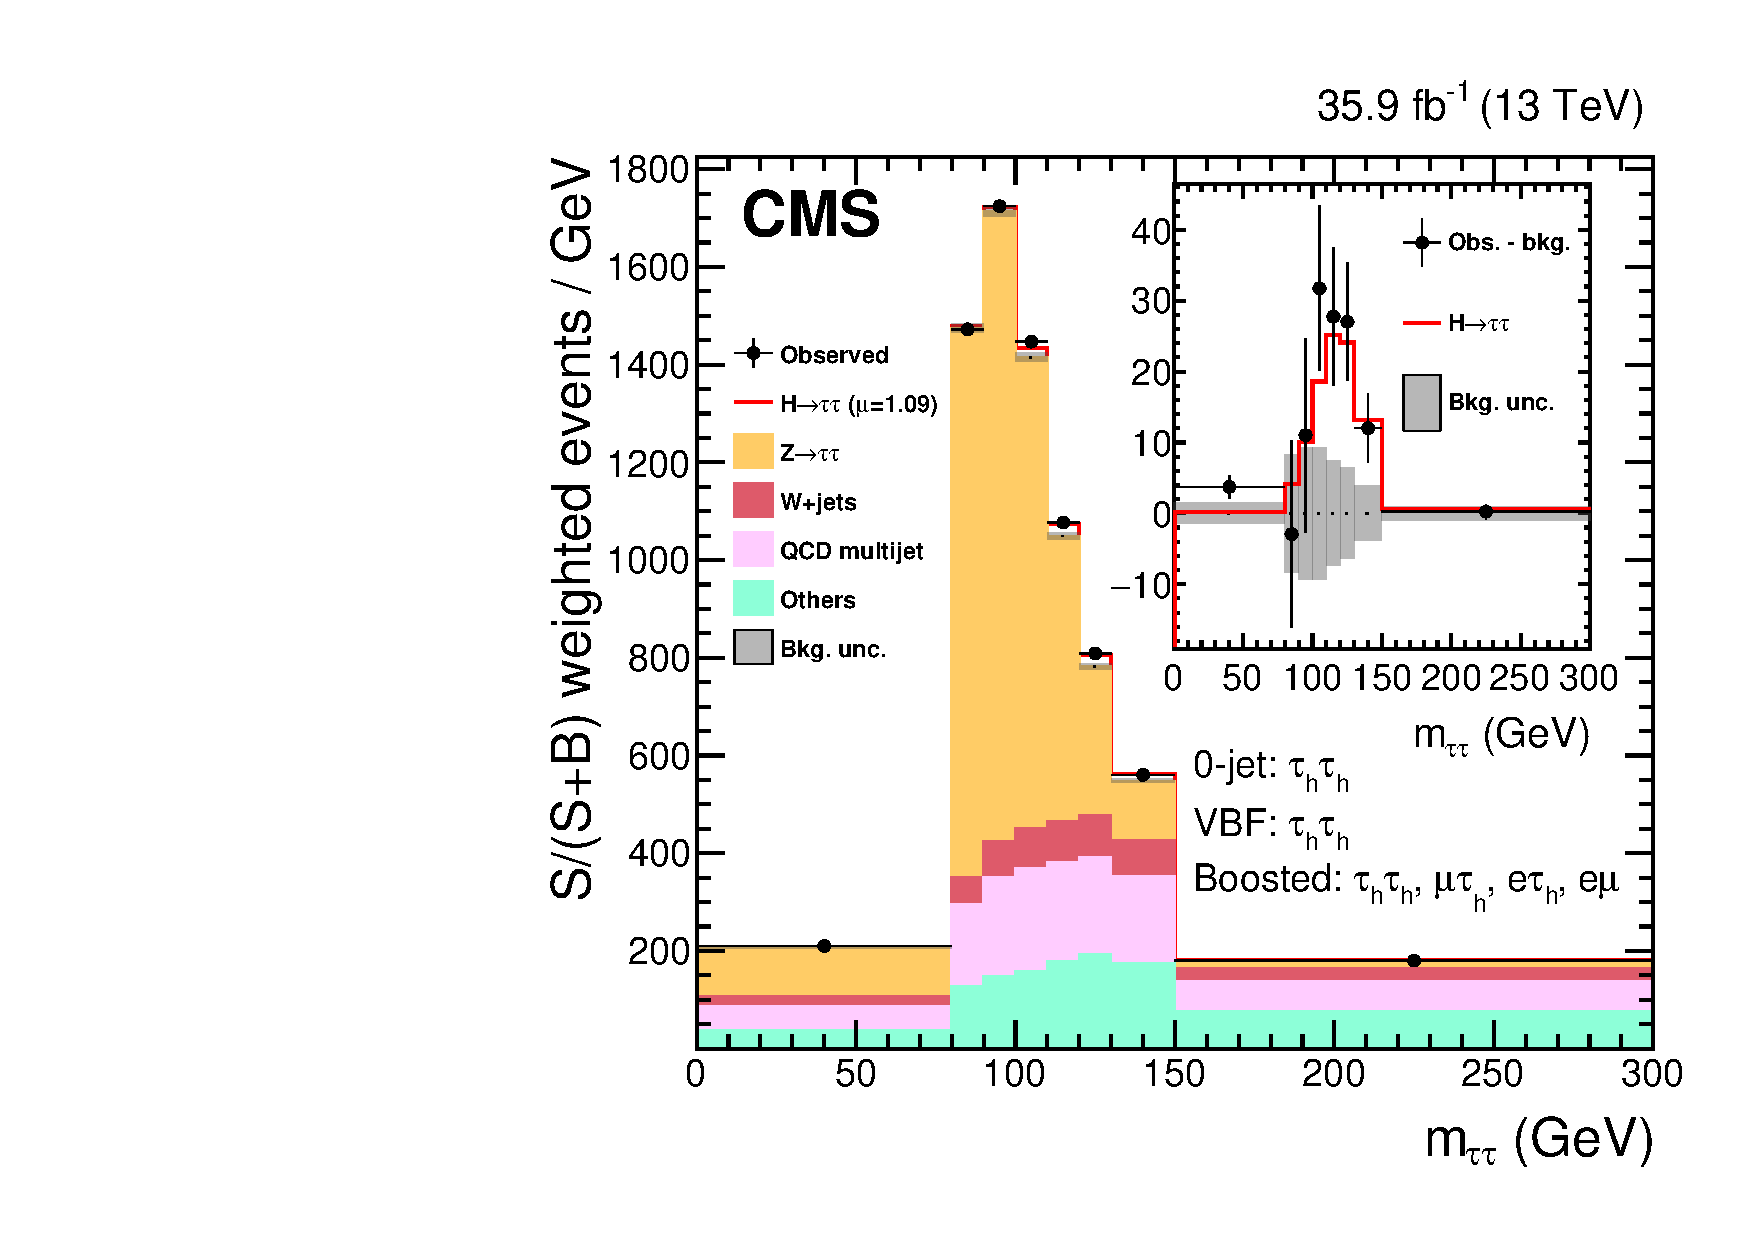
\includegraphics[width=0.48\textwidth]{figures/Figure_019-b.pdf}
   \caption{Combined observed and predicted $\mtt$ distributions. The left pane includes the VBF category of the $\Pgm\tauh$, $\Pe\tauh$ and $\Pe\Pgm$ channels, and the right pane includes all other channels that make use of $\mtt$ instead of $\mvis$ for the signal strength fit. The binning reflects the one used in the 2D distributions, and does not allow merging of the two figures. The normalization of the predicted background distributions corresponds to the result of the global fit, while the signal is normalized to its best fit signal strength. The mass distributions for a constant range of the second dimension of the signal distributions are weighted according to $S/(S+B)$, where $S$ and $B$ are computed, respectively, as the signal or background contribution in the mass distribution excluding the first and last bins. The ``Others" background contribution includes events from diboson, $\ttbar$, and single top quark production, as well as Higgs boson decay to a pair of $\PW$ bosons and $\PZ$ bosons decaying to a pair of light leptons. The background uncertainty band accounts for all sources of background uncertainty, systematic as well as statistical, after the global fit. The inset shows the corresponding difference between the observed data and expected background distributions, together with the signal expectation. The signal yield is not affected by the reweighting.
   }
    \label{fig:massweighted}

\end{figure}

The excess in data is quantified by calculating the corresponding local $p$-value using a profile likelihood ratio test statistic~\cite{LHC-HCG-Report,Chatrchyan:2012tx,Junk,Read:2002hq}.
As shown in Fig.~\ref{fig:pvalue}, the observed significance for a SM Higgs boson with $\mH = 125.09$\GeV is 4.9 standard deviations, for an expected
significance of 4.7 standard deviations.

\begin{figure}[!ht]
  \centering
    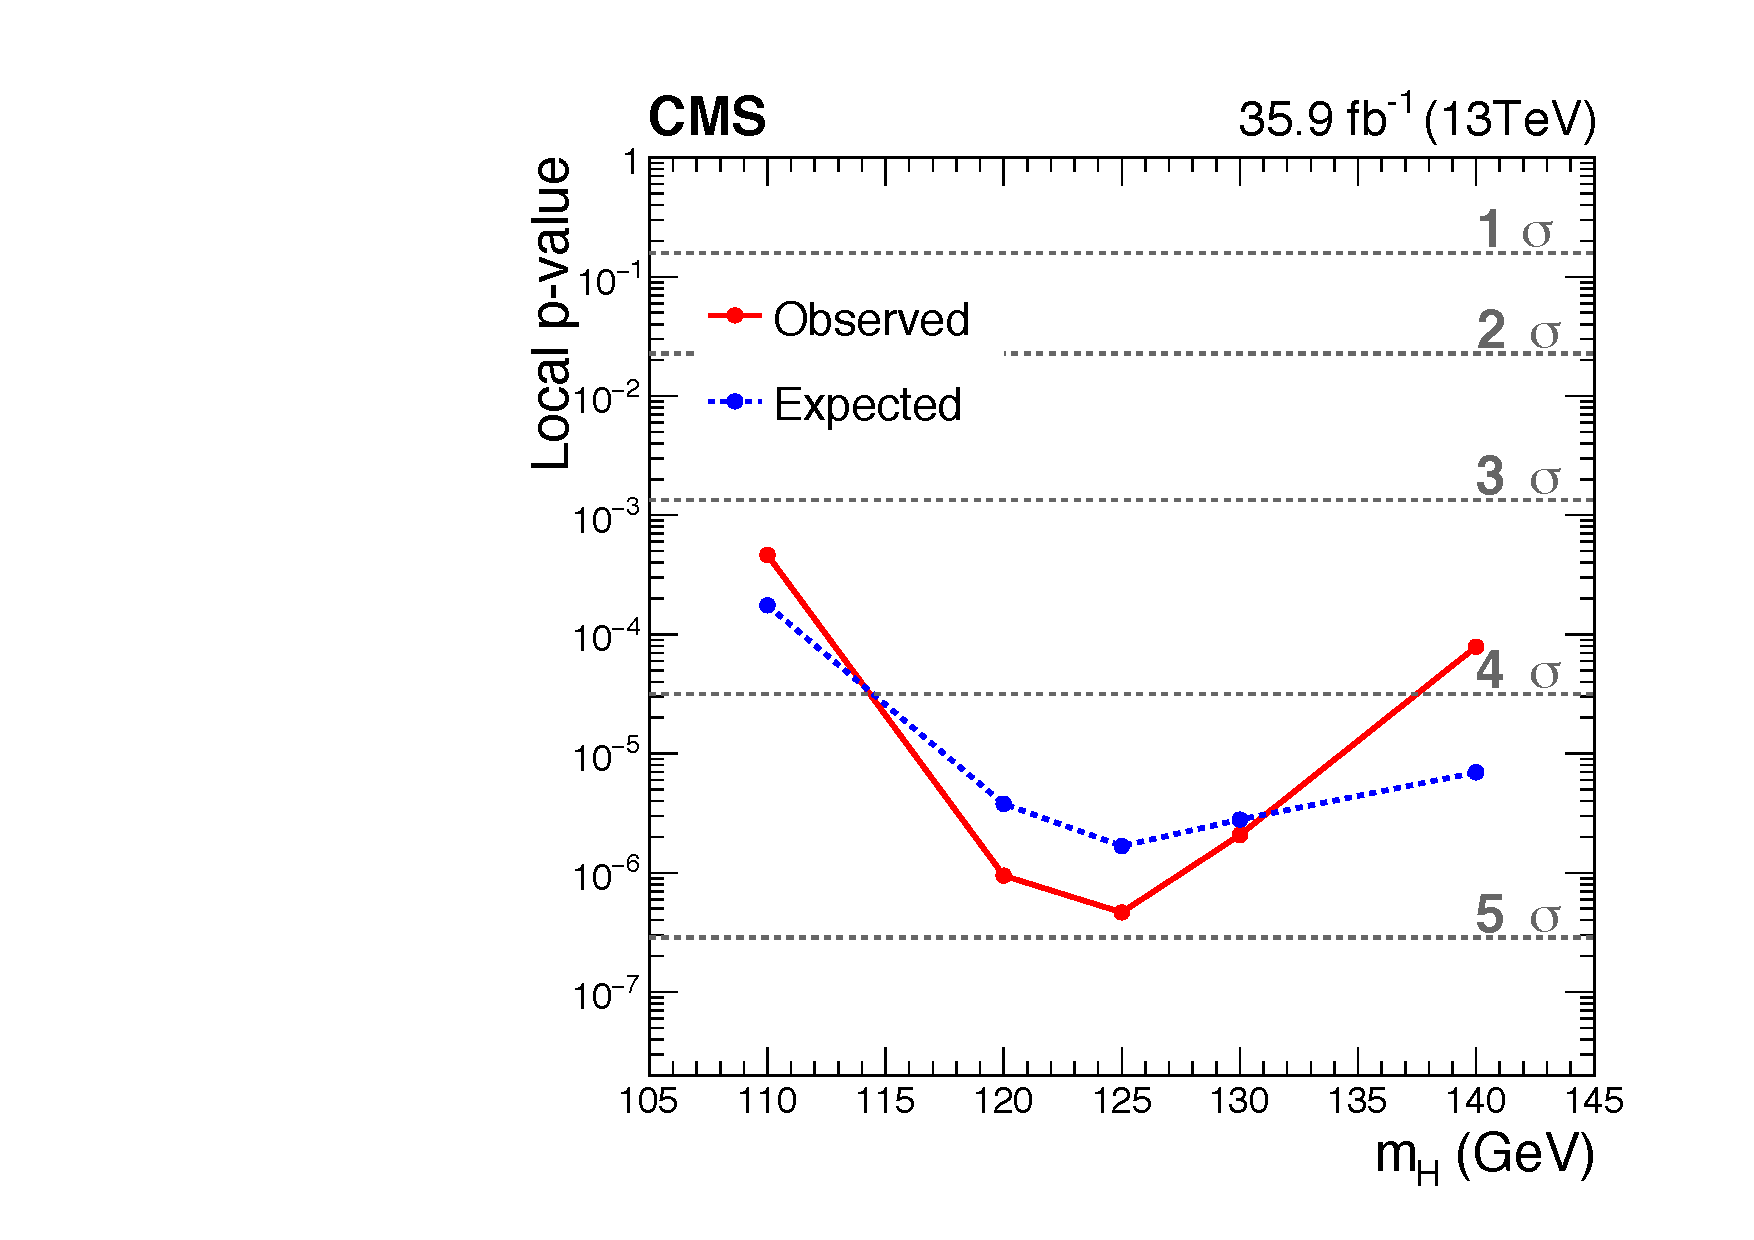
\includegraphics[width=0.5\textwidth]{figures/Figure_020.pdf}
   \caption{Local ${p}$-value and significance as a function of the SM Higgs boson mass hypothesis. The observation (red, solid) is compared to the expectation (blue, dashed) for a Higgs boson with a mass $\mH = 125.09$\GeV. The background includes Higgs boson decays to pairs of $\PW$ bosons, with $\mH = 125.09$\GeV.}
    \label{fig:pvalue}

\end{figure}


The corresponding best fit value for the signal strength $\mu$ is $1.09 ^{+0.27} _{-0.26}$ at $\mH = 125.09\GeV$. The uncertainty in the best fit signal strength can be decomposed into four components: theoretical uncertainties, bin-by-bin statistical uncertainties on the backgrounds, other systematic uncertainties, and the statistical uncertainty. In this format, the best fit signal strength is $\mu = 1.09^{+0.15}_{-0.15}\stat{}^{+0.16}_{-0.15}\syst{}^{+0.10}_{-0.08}\thy{}^{+0.13}_{-0.12}$ (bin-by-bin).
The individual best fit signal strengths per channel and per category, using the constraints obtained on the systematic uncertainties through the global fit, are given in Fig.~\ref{fig:muvalue}; they demonstrate the channel- and category-wise consistency of the observation with the SM Higgs boson hypothesis.

\begin{figure}[!ht]
  \centering
    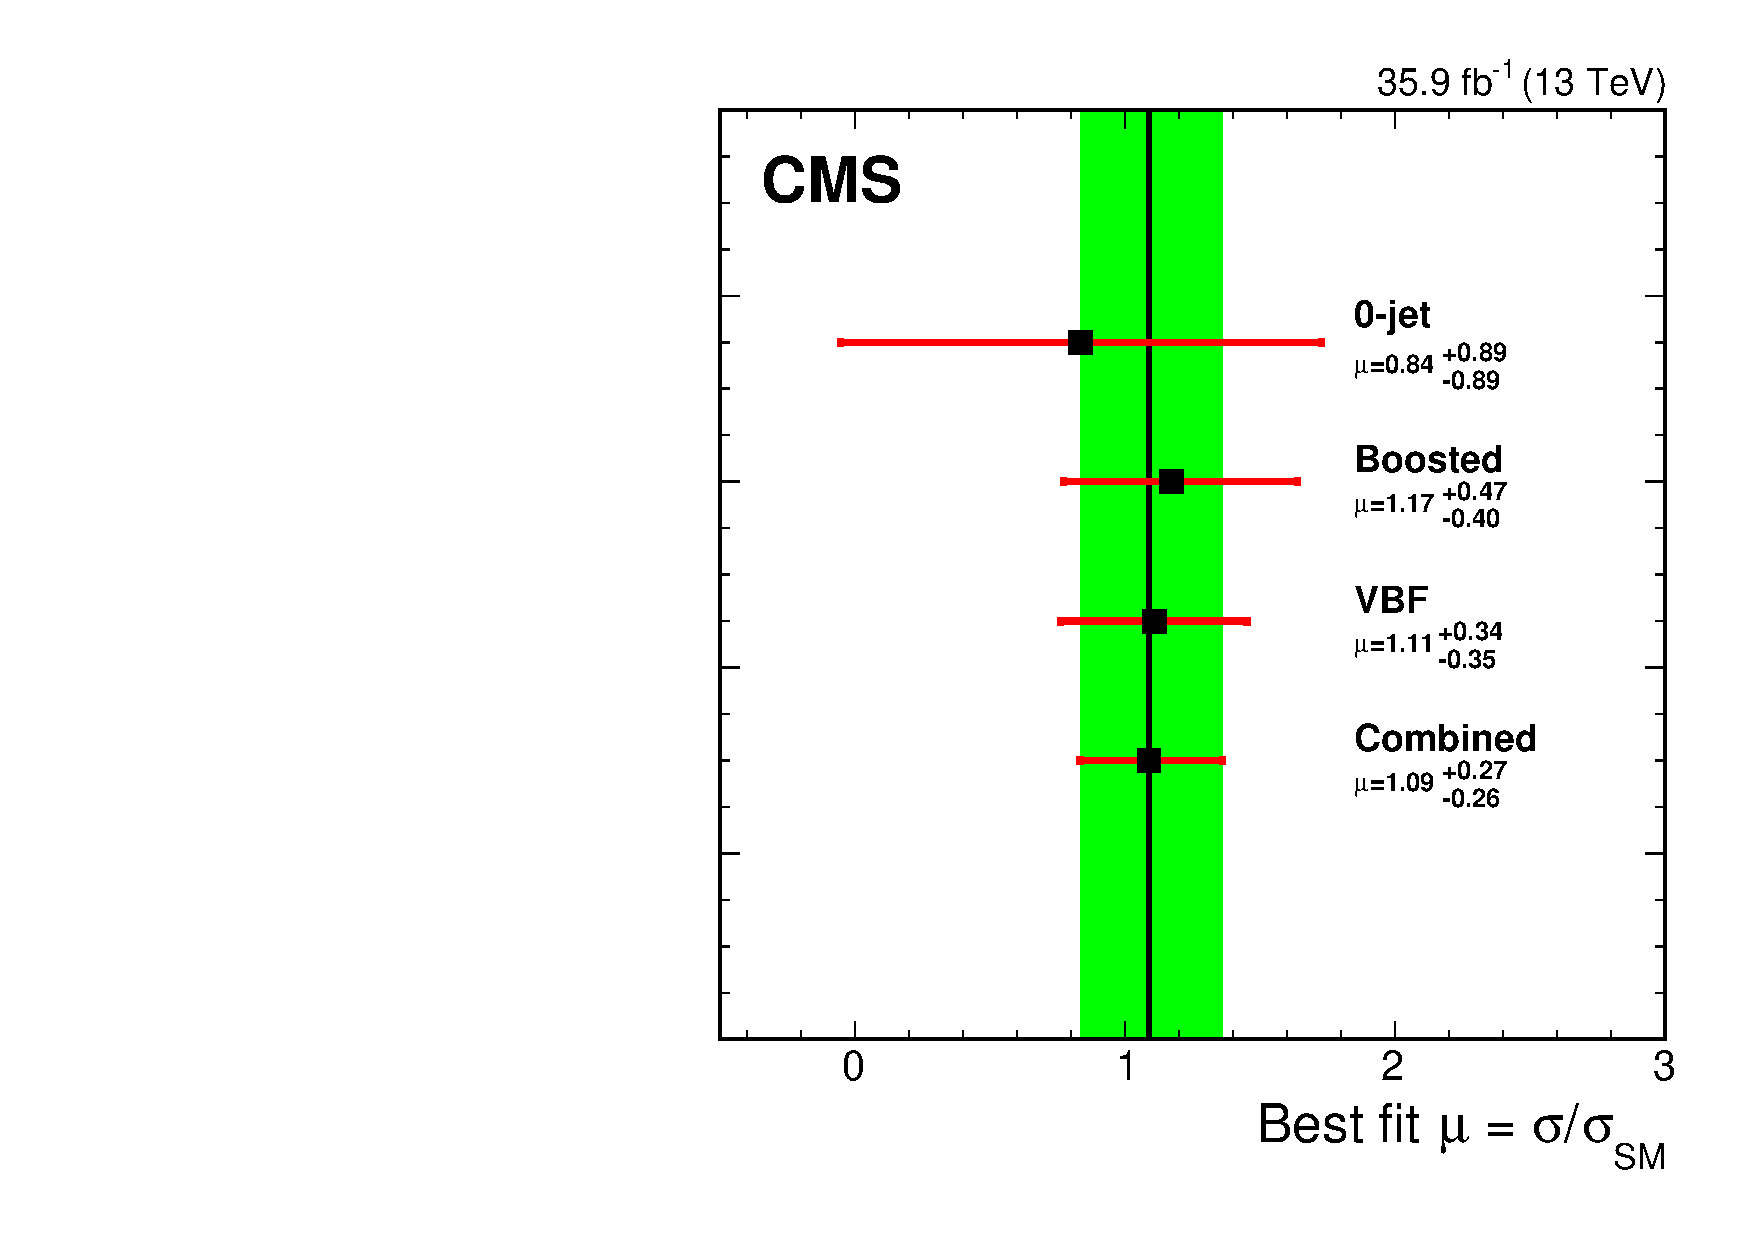
\includegraphics[width=0.49\textwidth]{figures/Figure_021-a.pdf}
    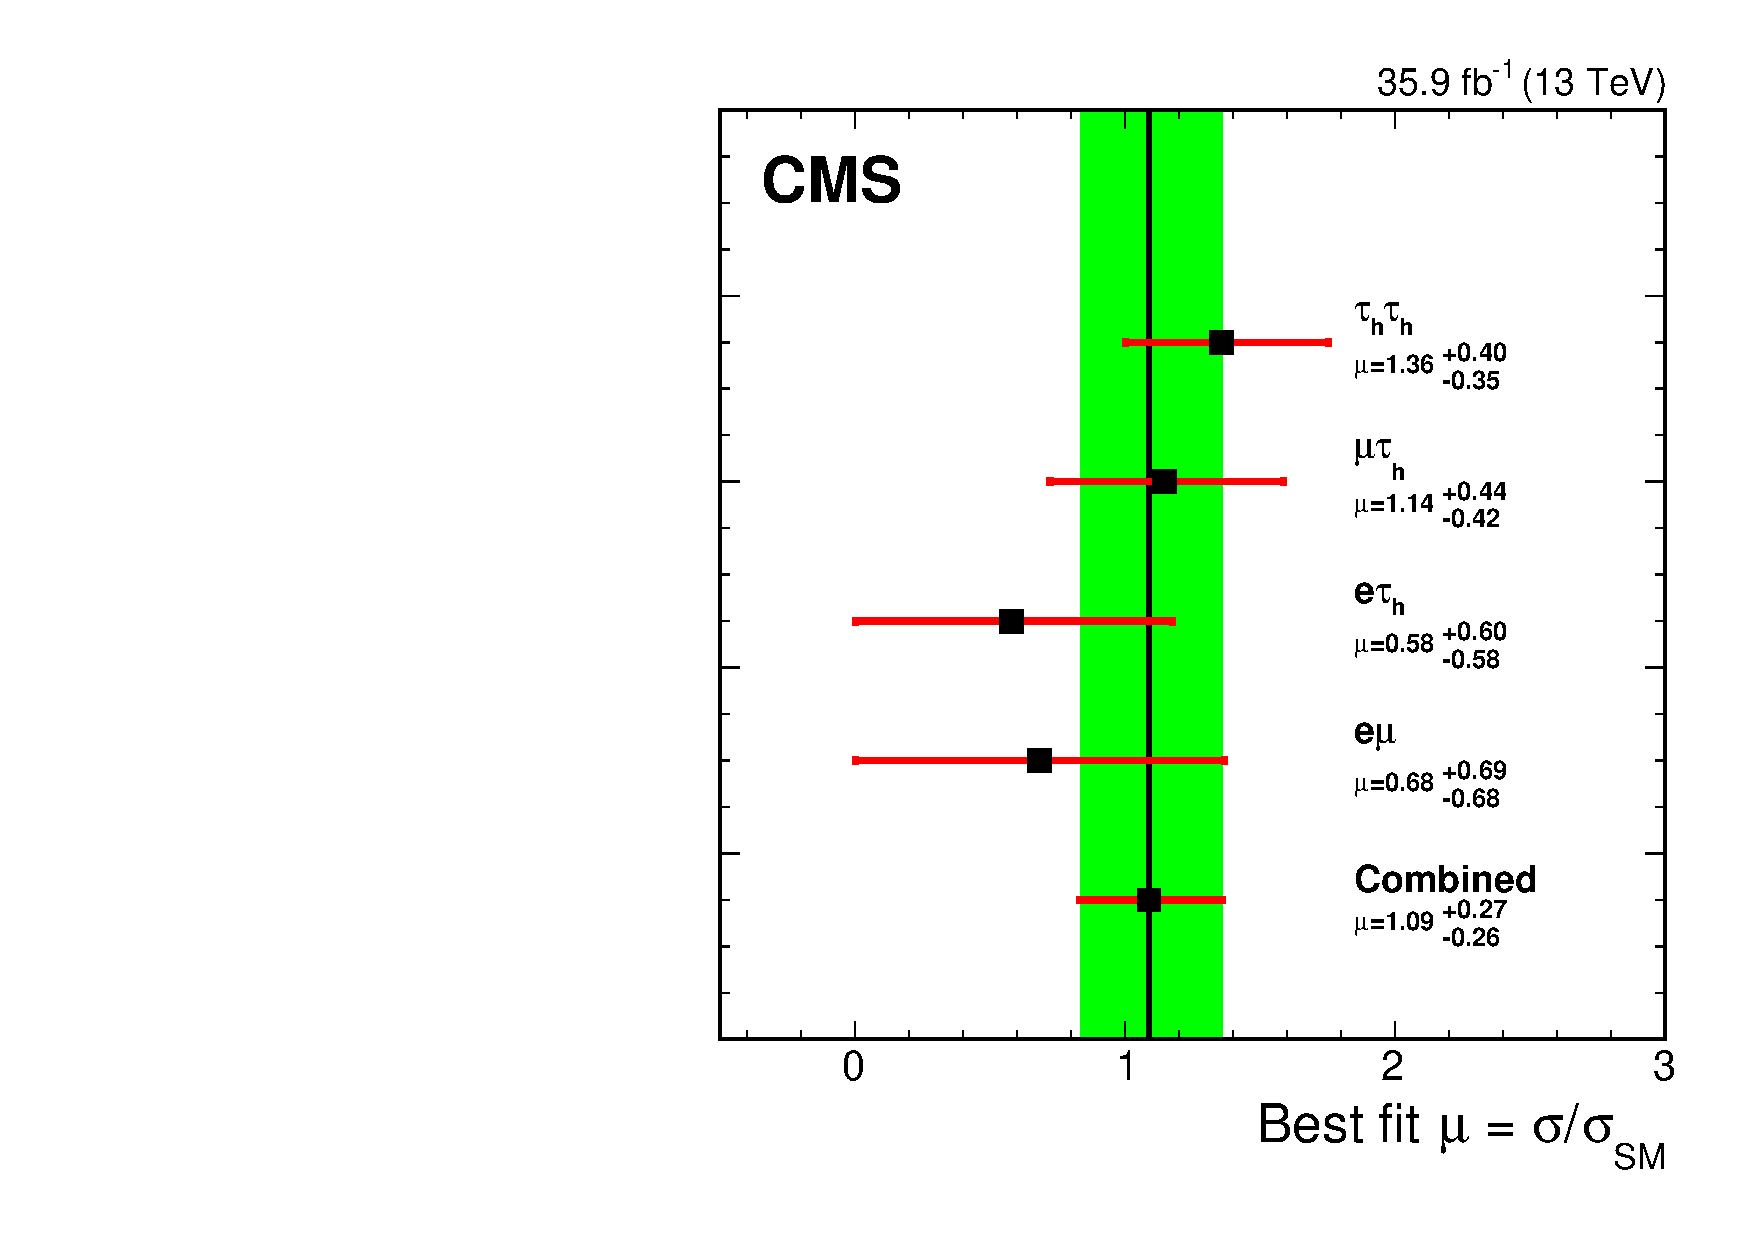
\includegraphics[width=0.49\textwidth]{figures/Figure_021-b.pdf}
   \caption{Best fit signal strength per category (left) and channel (right), for $\mH = 125.09$\GeV. The constraints from the global fit are used to extract each of the individual best fit signal strengths. The combined best fit signal strength is $\mu = 1.09 ^{+0.27} _{-0.26}$.}
    \label{fig:muvalue}

\end{figure}

A likelihood scan is performed for $\mH=125.09$\GeV in the ($\kappa_\mathrm{V}$,$\kappa_\mathrm{f}$) parameter space, where $\kappa_\mathrm{V}$ and $\kappa_\mathrm{f}$ quantify, respectively, the ratio between the measured and the SM value for the couplings of the Higgs boson to vector bosons and fermions, with the methods described in Ref.~\cite{Chatrchyan:2014nva}. For this scan only, Higgs boson decays to pairs of $\PW$ bosons are considered as part of the signal. All nuisance parameters are profiled for each point of the scan. As shown in Fig.~\ref{fig:kVkf}, the observed likelihood contour is consistent with the SM expectation of $\kappa_\mathrm{V}$ and $\kappa_\mathrm{f}$ equal to unity.


\begin{figure}[!ht]
  \centering
    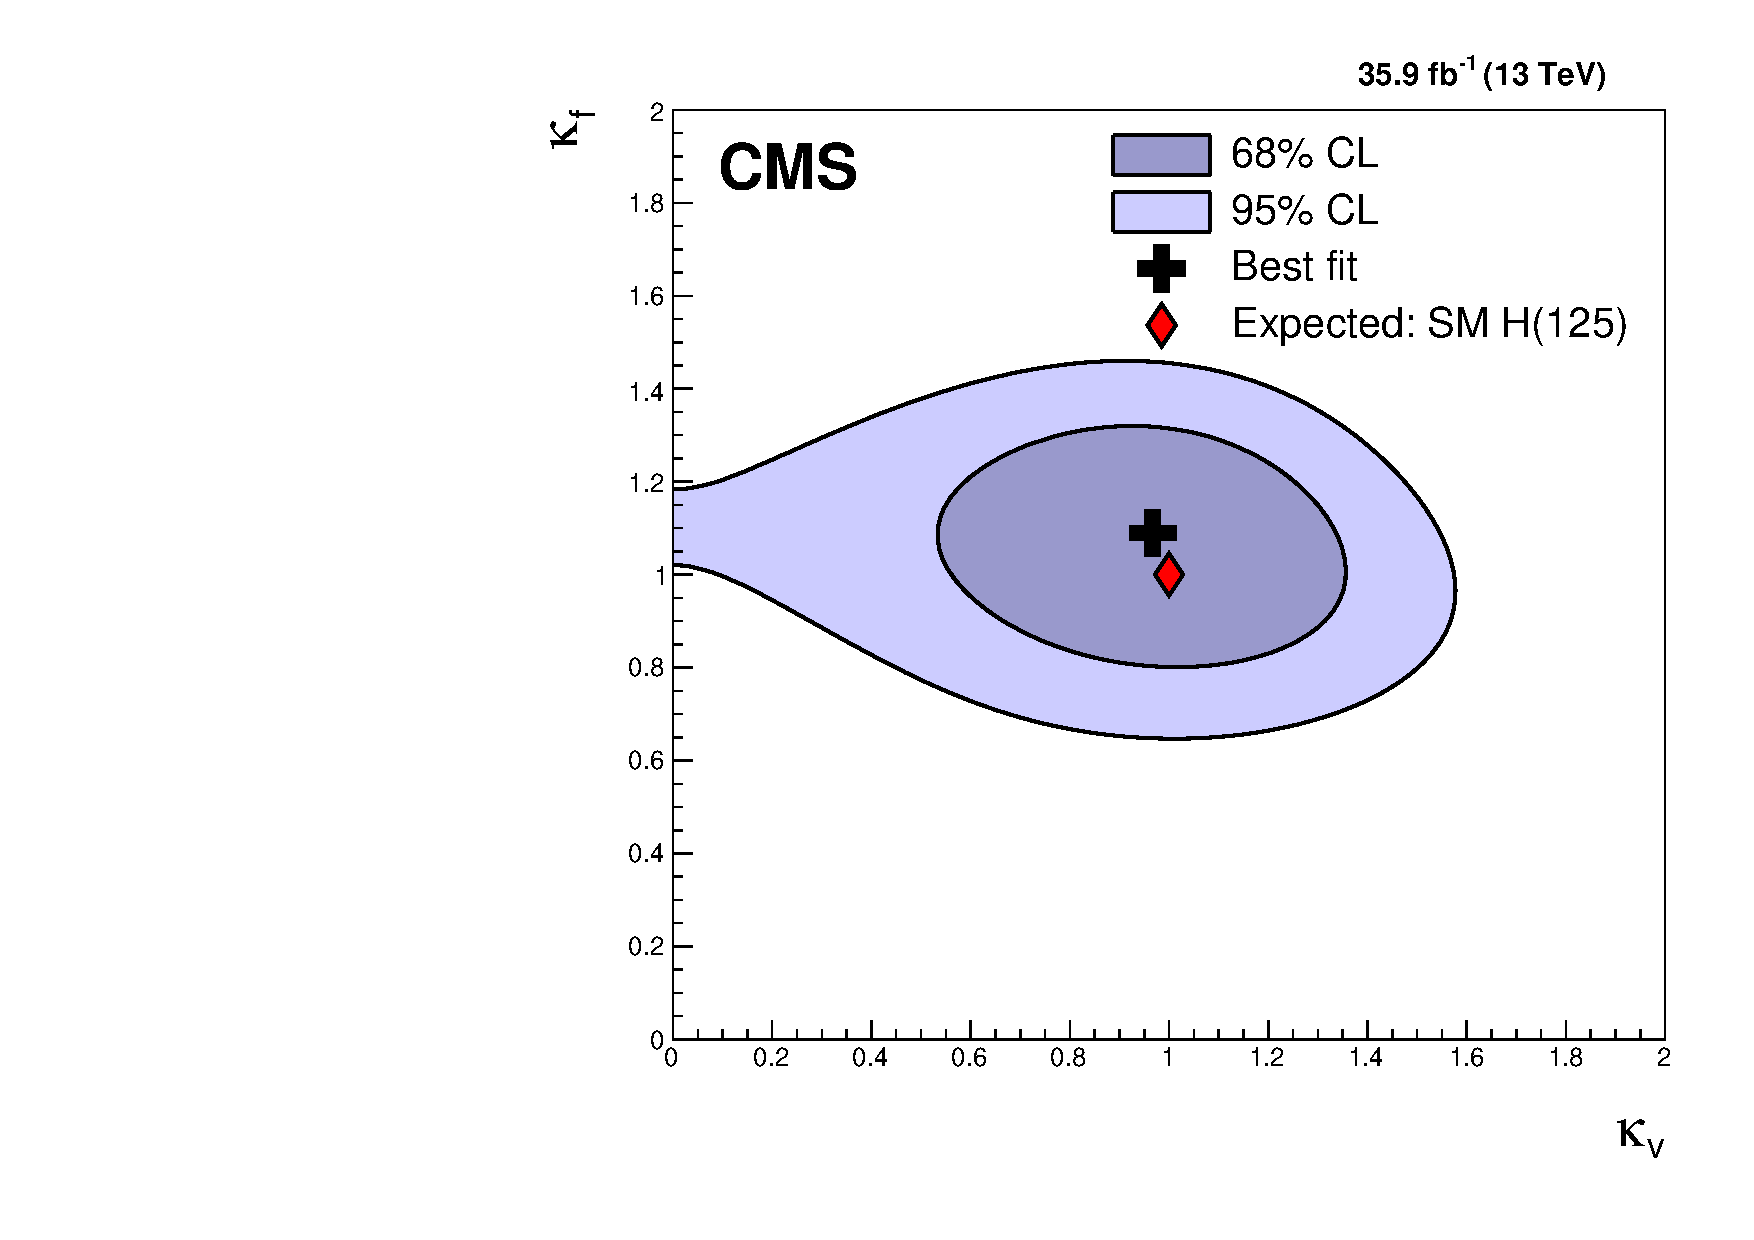
\includegraphics[width=0.65\textwidth]{figures/Figure_022.pdf}
   \caption{Scan of the negative log-likelihood difference as a function of $\kappa_V$ and $\kappa_f$, for $\mH = 125.09$\GeV.  All nuisance parameters are profiled for each point. For this scan, the $\Pp\Pp\to \PH\to\PW\PW$ contribution is treated as a signal process.}
    \label{fig:kVkf}

\end{figure}

The results are combined with the results of the search for $\PH\to\Pgt\Pgt$ performed with the data collected with the CMS detector at center-of-mass energies of 7 and 8\TeV~\cite{Khachatryan:2014jba}, using a common signal strength for all data taking periods. All uncertainties are considered as fully uncorrelated between the different center-of-mass energies. The combination leads to an observed and an expected significance of 5.9 standard deviations. The corresponding best fit value for the signal strength $\mu$ is $0.98\pm 0.18$ at $\mH = 125.09\GeV$. This constitutes the most significant direct measurement of the coupling of the Higgs boson to fermions by a single experiment.

\subsection{Signal Strength}
\subsubsection{$\mu$ By Channel}
\subsubsection{$\mu$ By Category}
\subsubsection{$\mu$ Combined}
\subsection{Significance Scan}
\subsection{Higgs Couplings}
kappaF kappaV plot
\subsection{Decomposition of Impact of Uncertainties}

\section{ZHiggs to $\ell\ell\tau\tau$}

\subsection{Signal Strength}
\subsubsection{$\mu$ By Channel}
\subsubsection{$\mu$ By Category}
\subsubsection{$\mu$ Combined}
\subsection{Higgs Couplings}
kappaF kappaV plot

\section{Combined}

\subsection{Signal Strength}
\subsubsection{$\mu$ By Process}
\subsubsection{$\mu$ Combined}
\subsection{Higgs Couplings}
kappaF kappaV plot

